\documentclass{xdupgthesis}
\usepackage{theorem}
\usepackage{siunitx}
\usepackage{amssymb}
\usepackage{bbding} 
\usepackage{graphicx}
\usepackage{algorithm}
\usepackage{tabularray}
\usepackage{booktabs}
\usepackage{subcaption}
\usepackage{diagbox}
\usepackage{makecell}
\usepackage{titlesec}

% 定义 mysubsubsection 标题格式
% \titleformat{\subsubsection}[block]{\normalsize\normalsize}{(\arabic{subsubsection})}{0.5em}{}[]



\usepackage[noEnd=false]{algpseudocodex}
\xdusetup {
  info/title = {基于混合专家网络与目标特征融合的点云姿态识别技术研究},
  info/title* = {Research on Point Cloud Pose Recognition Technology\\Based on Mixture of Experts Network and Target Feature Fusion},
  info/clc = TP39,
  info/keywords = {姿态识别,深度学习,毫米波雷达,混合专家网络},
  info/keywords* = {Point Cloud Registration, Deep Learning, Millimeter Wave Radar, Constant False Alarm Rate},
  info/graduate-type = 硕士,
  info/degree-type = 专业,
  info/degree = 电子信息硕士,
  info/degree* = Electronic Information,
  info/domain = 计算机技术,
  info/author = {杨丽},
  info/author* = {Yangli},
  info/student-id = 22031212262,
  info/supervisor = 姜晓鸿,
  info/supervisor* = Jiang Xiaohong,
  info/supv-title = 教授,
  info/supv-title* = Professor,
  info/supv-ent =  崔西宁,
  info/supv-ent* =  Cui Xining,
  info/supv-ent-title = 研究员,
  info/department = {广州研究院},
  info/supv-ent-title* = Research Fellow,
  info/abstract = {chapters/abstract-cn.tex},
  info/abstract* = {chapters/abstract-en.tex},
  info/bio = {chapters/resume.tex},
  info/acknowledgements = {chapters/thanks.tex},
  info/los = {chapters/los.tex},
  info/loa = {chapters/loa.tex},
  info/bib-resource={chapters/references.bib},
  style/customize-edubg = false,
  style/customize-resresult = false,
  style/cjk-font = win,
  style/latin-font = tac,
  style/customize-los = true,
  style/customize-loa = true,
  style/math-font = libertinus,
  style/anonymous = false,
  style/ref-add-space = false,
  % style/remove-page ={声明页,致谢},
}

% 将默认的Require/Ensure自定义为Input/Output
\renewcommand{\algorithmicrequire}{\textbf{Input:}}
\renewcommand{\algorithmicensure}{\textbf{Output:}}



\begin{document}

\chapter{绪论}

\section{研究背景与意义}


毫米波雷达作为一种先进的感知技术,在自动驾驶、无人机导航、智能交通系统和工业自动化等领域获得了广泛关注。它具有高分辨率、强穿透能力和良好的环境适应性,即使在雨雪、雾霾等恶劣天气条件下也能稳定工作。《新能源汽车产业发展规划(2021—2035年)》\cite{xbngyrqiie2020}指出,到2025年,新能源汽车新车销售量将达到汽车新车销售总量的20\%左右,自动驾驶的安全水平将全面提升,车载毫米波雷达和激光雷达将成为L2及以上自动驾驶的标配。

激光雷达由于其工作原理,性能常受光照变化和恶劣天气影响。相比之下,毫米波雷达在光照变化、烟雾、雾霾等能见度低的条件下依然能有效工作。尽管毫米波雷达生成的点云数据较为稀疏且噪声较高,但在这些条件下依然能够感知外部环境\cite{qian20203d},成为自动驾驶和环境监测中的重要技术。

点云是一种数据表示形式,主要用于3D建模或测量领域,每个点在空间中表示一个具体的位置。使用点云数据描述物体的方式广泛应用于捕捉和表现物理世界中的各种形状和场景。

点云配准是将多个点云数据集整合到一个统一的坐标系统中的过程。例如,在自动驾驶领域,通过点云配准,车辆能够更准确地识别和定位周围的物体和环境特征,实现更安全的导航。在环境建模方面,通过配准不同视角和位置的点云数据,可以创建出精确的三维模型用于进一步的分析和可视化处理。到目前为止,学术界和工业界已有大量适用于非毫米波雷达的配准方案。

由于毫米波雷达能在激光雷达无法工作的情况下保持正常运作,研究适合毫米波雷达点云数据的检测与配准方案变得尤为重要。在毫米波雷达点云配准中,存在两个待解决的主要问题。首先,由于毫米波雷达的工作频率较低,通常会产生较高水平的噪声。在低信噪比、多目标的情况下,使用恒虚警率(Constant False Alarm Rate,CFAR)算法\cite{7185}生成毫米波雷达点云中的目标点时,存在性能退化和无法有效提取目标点的问题。因此,如何在噪声环境中准确地识别和检测出目标点面临严峻挑战。
其次,毫米波雷达获取的点云数据往往比较稀疏,并且点的密度不均匀。而稀疏以及不均匀性可能导致适用于激光雷达的传统配准方案在毫米波雷达点云配准过程中出现位置偏差或配准不精确的问题,进而影响到自动驾驶、环境监测等应用的性能和可靠性。因此,需针对噪声干扰和点云稀疏性的研究有效配准算法,以确保毫米波雷达点云数据能够准确地在不同坐标系下进行配准和使用。

\section{研究面临的问题}
毫米波雷达点云不同于激光雷达点云,由于其工作频率较低、受噪声干扰较大,导致难以检测出有效目标点数据,且目标点形成的点云数据具有稀疏、密度不均匀的特点。

\textbf{问题一:存在未知的噪声干扰,难以有效检测目标点}
\par
在毫米波雷达工作时,收到的回波信号除了有效目标点的信息,还包括路边建筑的反射、目标的多次反射、多径效应等带来的噪声\cite{richards2010principles}。噪声的干扰导致在提取毫米波雷达点云的有效目标点时会产生虚假点云。由于传统的CFAR算法在处理毫米波雷达回波信号时,只能关注有限的训练单元,导致CFAR算法在判断距离多普勒图中是否有目标存在时,只能考虑到特定的局部信息,而无法全面考虑整个场景的复杂情况,在低信噪比、多目标的情况下,会因为虚假点云而导致检测目标点的性能下降。
\par
\textbf{问题二:毫米波雷达点云密度稀疏且不均匀,传统配准算法难以工作}
\par
点云配准算法,如迭代最近点(Iterative Closest Point,ICP)算法\cite{besl1992method}等对于待配准点云要求有明显可识别的特征,这些特征在配准过程中用于识别对应的点,此外配准的效果依赖点云中点的数量,需要大量的点信息提高配准效果。毫米波雷达在工作时使用扫描的方式,在靠近雷达处扫描到的点云较为稠密而远离雷达处的点云较为稀疏,使得在多个不同位置工作的毫米波雷达对于统一物体扫描所得到的点云稀疏程度不一致,导致对于同一物体特征的识别变得困难。毫米波雷达工作频率较低、波长较长的特征使毫米波雷达拥有了更强的穿透力和检测距离,但是这也导致了范围分辨率较低。60GHz的毫米波雷达距离分辨率约为3.75cm\cite{meta2007signal},而激光雷达的分辨率可以达到毫米级,毫米波的原理决定了其点云无法达到激光雷达的分辨率。点云密度不均匀和点云密度稀疏的问题导致传统配准算法难以工作。
\section{国内外研究现状}
在上述研究背景下,本节对毫米波雷达回波信号目标点检测方案和毫米波雷达点云配准方案当前的国内外研究现状进行了总结和分析。
\subsection{毫米波雷达目标点检测}
目前雷达回波信号目标点检测算法主要分为两大类,基于检测单元平均值统计评估的CFAR算法以及CFAR算法的改进和基于深度学习的点云目标点检测。

\par
(1)传统目标点检测方法
\par
传统的雷达回波信号目标检测大多是基于CAFR算法的改进,此类算法主要方法是根据参考单元杂波噪声识别进行评估得到平均背景噪声水平,根据虚警率计算阈值因子,使用阈值因子与平均背景噪声水平相乘以得到检测阈值的恒定虚警率检测算法。最早的CFAR算法是单元平均恒虚警率算法(Cell Average CFAR,CA-CFAR)\cite{4043676},CA-CFAR利用周围参考单元的平均值作为噪声水平的评估。然而,CA-CFAR在多目标以及非均匀噪声的环境下检测效性能会急剧下降。对CA-CFAR改进的算法有最大平均恒虚警率算法( Greatest of CFAR,GO-CFAR)\cite{4102285}和最小平均恒虚警率算法(Smallest of CFAR,SO-CFAR)\cite{trunk1978range}。GO-CFAR可以良好地控制虚警率但是在多目标情况下无法正确评估噪声水平。SO-CFAR在多目标环境的目标点检测有良好的效果,但是无法良好地控制虚警率。为改进基于平均值的CFAR在多目标场景下的检测性能下降,Rohling提出了基于有序统计的CFAR检测算法( Ordered Statistic CFAR,OS-CFAR)\cite{4102829},通过将排序后的第k个值作为背景噪声水平估计值计算检测阈值。但是OS-CFAR的k值选择会极大的影响检测性能。Wang等人提出了一种新的密度审查操作\cite{WangCFAR},在局部 CFAR 检测之前快速识别去除大量无信息背景杂波,减少了后续CFAR检测的计算成本以及由此产生的误报数量。但是这些方法都无法有效解决多目标时目标点误报问题。

\par
(2)基于深度学习的目标点检测方法
\par
基于深度学习目标检测技术,依托于神经网络对特征的提取和抽象能力,为毫米波雷达的目标点检测提供了新的思路\cite{mata2015mlp}。
Akhtar等人以OS-CFAR为基础,提出了使用多层MLP神经网络辅助OS-CFAR设置动态阈值的方案\cite{akhtar2021training}。
Kang等人提出了基于Faster R-CNN的检测方案\cite{R-CNN-CFAR},该方案使用Faster R-CNN生成CFAR算法的保护单元,优化了小目标检测性能。Lin等人提出了基于卷积神经网络的CFAR方案\cite{DL-CFAR},降低了多目标场景中掩蔽效应的影响,在信噪比的情况下表现良好。
Faruk等人提出了基于CNN\cite{lecun1989backpropagation}的毫米波雷达目标点检测RadCNN\cite{CNN-CFAR},该方案使用分块输入距离多普勒图到CNN的方式返回预测后的分块结果。
Cao等人提出了基于DNN\cite{DBLP:conf/nips/KrizhevskySH12}的毫米波雷达峰值检测方案\cite{DNN-CFAR},该方案将目标点检测问题转化为频率强度序列分类问题。
Cheng等人提出了避免虚假点的新方案\cite{9823311},设计了一个编码器-解码器的网络,使用的标签为LiDAR检测数据。编码器的输入为距离多普勒图,解码器的输出为一个预测标签的矩阵,表示在距离多普勒图上的每个单元是否为目标点。但是该方案需要使用LiDAR配套生成训练数据,且LiDAR数据没有多普勒维度,用于对距离多普勒图做预测的效果不佳。
Zhao等人,提出了使用DBSCAN\cite{schubert2017dbscan}结合ANN网络\cite{agatonovic2000basic}的方案,使用DBSCAN聚类排除目标附近因为旁瓣效应带来的干扰峰值,使用ANN估计背景噪声的参数\cite{sym11121482}。但是该方案因为引入了DBSCAN导致计算需要花费更多的时间,并且在低信噪比的情况下性能会降低。
Akarsh的方案RadarHD\cite{10161429}与上面的方案不同,不再使用传统的快速傅里叶变化(Fast Fourier Transform,FFT)处理后的距离多普勒图来检测有效目标点,而是设计了一个端到端的神经网络,使用雷达原始的I/Q数据作为输入,使用激光雷达对同一片环境的稠密点云作为标签训练了点云生成网络。该方案虽然能够生成高质量点云,但是需要激光雷达的数据作为标定,适用性不强。
\subsection{毫米波雷达点云配准}

\par
(1)传统点云配准
\par
传统的点云配准方案如迭代最近点、核心相关(Kernel Correlation,KC)\cite{DBLP:journals/cad/SongHDLY22}、鲁棒点匹配(Robust Point Matching,RPM)\cite{ma2014robust}等,通过匹配源点云和参考点云的特征点,迭代计算出最优的配准变换矩阵以最小化点云之间的距离。ICP算法通过迭代优化对应点对之间的距离,实现点云的配准;RPM算法通过计算源点云和参考点云中点与点的对应关系,找到对应点对后进行配准;KC算法通过寻找待配准点云之间的相似性,找出最大相似性后计算出最优的变换矩阵以实现配准。然而,这些传统算法都在处理毫米波雷达点云时面临困难,因为毫米波雷达点云通常稀疏且易受噪声影响,使得传统算法的性能下降。

\par
(2)基于深度学习的点云配准
\par
检测到毫米波雷达目标点后,需要将多个雷达的目标点数据配准到同一个坐标系的点云下。由于毫米波雷达点云密度稀疏且不均匀的特性,许多专家学者在其点云的配准上进行了大量的研究。
Shastri等人提出了mmSCALE\cite{mmSCALE},通过利用环境中人员的运动轨迹自动估计多个雷达相对于参考坐标系的位置和方向,使用奇异值分解(Singular Value Decomposition,SVD)最小二乘法(Least Sqaure Method,LS)获取毫米波雷达的相对位置和方向。但是此方案所适用场景为毫米波雷达部署之前,预先估计出坐标变化,不适用于已有点云数据的配准。
Chen等人\cite{9827800}提出了通过标记的方式配准点云。通过预先设置标记点并构建其点云数据,自动泊车系统能够在运行过程中利用多帧融合技术准确捕获这些标记点的特征,借助标记点特征完成配准。此方案精度较高但是在无法安装标记点的场景无法使用。
Yeong等人提出了在低能见度的情况下,使用毫米波雷达生成点云的方案\cite{8967633}。其方案使用预先构建的密集 LiDAR 点云辅助毫米波雷达雷达测量结果以进行定位,在激光雷达无法工作的环境使用毫米波雷达点云数据依据预先构建的激光雷达图,通过点云配准感知如浓雾等环境中的情况。但是该方案依赖于使用激光雷达先进行地形图的扫描,使用比较局限。Yew等人提出了使用PointNet\cite{qi2017pointnet}提取点云特征的方案\cite{Yew_2020_CVPR},Xiang等人提出了使用DBSCAN\cite{DBLP:conf/kdd/EsterKSX96}进行空间聚类进行特征提取的方案\cite{DBLP:journals/iotj/XiangMTYWGCKY24},这两个方案提高了提取单个点特征的丰富程度,但是无法克服点云密度不均匀带来的特征在密度不同处不适用的问题。
\section{论文研究内容与主要工作}
在毫米波雷达工作过程中,存在低信噪比、多目标的情况下难以从距离多普勒图中检测出目标点,检测出的目标点较为稀疏且分布不均匀,导致点云难以配准的问题。本文分析了现有的毫米波雷达目标点检测方案以及现有点云配准方案,结合毫米波雷达工作特点对如何有效检测目标点、如何对检测出的目标点进行有效配准做了深入研究,本文的研究内容如下:
\par
\textbf{研究内容一}:针对在低信噪比、多目标的情况下难以从距离多普勒图中提取出检测点的问题,提出一种基于残差神经网络\cite{he2016deep}和自注意力机制\cite{vaswani2017attention}的距离多普勒图处理方案RA-CFAR(Residual Attention CFAR)。RA-CFAR使用残差神经网络作为距离多普勒图局部的特征提取模块,并且通过自注意力模块结合距离多普勒图局部的空间特征自估计目标点所在单元的检测阈值。距离多普勒图是调频连续波雷达用于检测目标速度和位置的重要手段,距离多普勒的两个维度分别为速度维FFT和距离维FFT,目标的速度和距离会在距离多普勒图上呈现尖峰的形式。为了有效提取出尖峰所在单元,许多研究人员采取众多方式,如使用训练单元平均值估计CA-CFAR、训练单元排序第k大值估计OS-CFAR、采用深度学习估计训练单元的方案等。为了解决距离多普勒图检测目标点位置时,尤其是多运动目标时难以设置CFAR的参数,导致无法有效检测到目标点的问题,RA-CFAR 使用自注意力模块结合距离多普勒图局部的空间特征提出自估计阈值检测目标点所在单元的方案。并且通过与四种常用算法对比,证明RA-CFAR在处理多目标和低信噪比距离多普勒图时具有良好的性能。
\par
\textbf{研究内容二}:针对检测出的目标点较为稀疏和分布不均匀,导致点云难以配准的问题,研究当前毫米波雷达配准的主流方案,包括使用SLAM的雷达轨迹定位配准方案\cite{grisetti2010tutorial}以及点云的经典配准算法。使用SLAM的方案需要引入复杂的SLAM算法进行姿态估计并且不适用于历史点云数据的配准。经典配准算法如ICP算法,RPM算法,CPD算法\cite{cpd}等面对毫米波雷达低分辨率、稀疏且不均匀的点云配准效果不佳。分析毫米波雷达点云的特点,在点级别提出结合点云邻域的多普勒特征以及多尺度邻域的点特征提取方案即点云邻域特征提取网络。为了在点级别挖掘出更多特征,在点局部拟合法平面计算出点的法向量作为特征信息的一部分,使用点云邻域特征提取网络提取多个半径的邻域特征进行融合作为目标点最终特征。为加快配准的收敛,提出全局配准参数预测网络,使用源点云与参考点云的全局特征推测初始配准参数。迭代配准中使用源点云与参考点云的特征距离代替空间距离,使用推测的配准参数进行迭代配准。通过实验验证在毫米波雷达的点云配准中多尺度邻域特征以及配准参数推测的有效性。

\section{论文结构安排}
本论文主要分为六个章节,文章结构如图\ref{fig:论文结构安排}所示,相关内容安排如下:
\par
第一章,绪论。本章分析了毫米波雷达点云配准的研究背景和意义,分析了毫米波雷达点云配准面临的问题,总结了国内外研究现状,提出了本文的研究内容与主要工作。
\par
第二章,相关理论技术研究。本章分三个部分分别介绍了毫米波雷达相关的知识,点云配准相关的知识,深度学习相关的知识。在毫米波雷达相关知识中介绍了调频连续波雷达的工作原理,距离多普勒图的特点,以及雷达回波信号的处理。在点云配准相关知识中介绍了点云配准的基本概念,点云配准的基本流程,以及点云配准的常用算法。在深度学习相关知识中介绍了深度学习的基本概念,残差神经网络的基本结构,自注意力机制的基本原理。为后续的研究工作提供了理论基础。
\par
第三章,基于距离多普勒图空间相关性的目标点检测方案。本章首先分析了距离多普勒图的特点,研究了传统CFAR算法在处理距离多普勒图时的局限性,通过分析距离多普勒图中目标点区域的特征,提出了基于残差神经网络和自注意力机制的距离多普勒图处理方案。最后通过实验验证了RA-CFAR在处理多目标和低信噪比距离多普勒图时具有良好的性能。
\par
第四章,基于多尺度邻域的毫米波点云配准方案。本章针对毫米波雷达点云配准的问题,结合毫米波雷达点云的低分辨率、稀疏、密度分布不均匀的特点分析了传统配准算法不适用与毫米波雷达点云的原因,提出了结合点云邻域多普勒特征以及多尺度邻域特征融合的点特征提取方案即点云邻域特征提取网络,和使用源点云与参考点云的全局特征推测初始配准参数的方案即全局配准参数预测网络。经过实验验证了在毫米波雷达的点云配准中多尺度邻域特征以及配准参数推测的有效性。
\par
第五章,原型系统的设计与实现。本章将介绍毫米波雷达点云提取优化方案和点云迭代优化配准方案的具体实现,包括系统的整体架构设计、系统的模块划分、系统的具体实现细节、系统的性能测试等。验证了本文提出的方案在实际场景中的有效性。
\par
第六章,总结与展望。总结本文的研究工作,并对未来的工作进行了展望。
\begin{figure}[htbp]
	\centering
	\includegraphics[width=0.95\linewidth]{figures/论文结构.pdf}
	\caption{论文结构安排}
	\label{fig:论文结构安排}
\end{figure}
\chapter{相关理论技术研究}
点云是在同一空间参考系下目标物体的空间分布的大量点集合,点云图像是最基础也是最常见的三维图像。点云配准是将多个来自不同传感器或不同时间、空间的点云数据进行对齐和融合的过程。毫米波雷达的点云配准,是结合毫米波雷达自身数据特征,将多个毫米波雷达位于不同空间位置获取的点云进行融合。借助多个毫米波雷达配准后的点云获取更全面并且一致的环境信息。
\section{调频连续波雷达相关技术}
调频连续波雷达(Frequency Modulated Continuous Wave,FMCW)\cite{brooker2005understanding}是一种采用频率调制技术的雷达系统,主要用于测距和速度测量。相较于传统脉冲雷达,FMCW雷达在发送连续波形的同时进行频率调制,实现了对目标距离和速度的同时测量。 FMCW雷达主要由三个部分组成:发射部分、接收部分和处理部分。发射部分发射信号,经过物体反射由接收部分接收后经过混频器放大到中频,由处理部分获取目标的距离和速度信息。FMCW雷达的原理如图\ref{fmcw}所示。

\begin{figure}[htbp]
	\centering
	% Requires \usepackage{graphicx}
	\includegraphics[width=0.5\textwidth]{figures/fmcw.pdf}\\
	\caption{FMCW雷达框图}
	\label{fmcw}
\end{figure}

\subsection{FMCW雷达测距}
合成器生成的信号称为Chrip信号,Chrip信号频率随时间线性变化,信号时域图和频域图如图\ref{chrip},通常发射信号的频率在一个较小的范围内变化。每次发送与接收到的回波信号与发射信号之间存在频率差。接收部分中的混频器用于将接收到的信号与本地振荡器的信号混频产生中频(Intermediate Frequency,IF)信号\cite{waters1982bandpass}。中频信号随时间的变化包含了目标的距离和速度信息。

\begin{figure}[htbp]
	\centering
	% Requires \usepackage{graphicx}
	\includegraphics[width=0.8\linewidth]{figures/Chrip信号时频域图}\\
	\caption{Chrip信号时频域图}
	\label{chrip}
\end{figure}

FMCW雷达在$t_1$时刻合成器合成频率为$f_1$的Chrip信号,经过物体对该信号的反射,生成一个由接收天线捕捉的信号。在经过延时$\tau$后由接收天线收到信号,混频器将收到的信号与发送信号混合,生成一个具有新频率的新信号。如公式\eqref{signal1}和\eqref{signal2}表示两个输入的正弦信号$x_1$和$x_2$。
\begin{equation}
	x_1 = \sin(\omega_1t+\Phi_1)
	\label{signal1}
\end{equation}
\begin{equation}
	x_2 = \sin(\omega_2t+\Phi_2)
	\label{signal2}
\end{equation}
经过混频器混合后得到$x_3$。
\begin{equation}
	x_3 = \frac{1}{2}\sin \big(\left(\omega_1 + \omega_2\right)t + \Phi_1+ \Phi_2\big) + 
	\frac{1}{2}\sin \big(\left(\omega_1 - \omega_2\right)t + \Phi_1- \Phi_2\big) 
\end{equation}
经过低通滤波后,得到如公式\eqref{signal_out}所示的中频信号$x_{out}$,其频率为$x_1$与$x_2$频率的差值。
\begin{equation}
	x_{out} = \frac{1}{2} \sin\big((\omega_1 - \omega_2)t + \Phi_1- \Phi_2\big)
	\label{signal_out}
\end{equation}
混频器的运行方式如图\ref{IF}所示,图像中两条线的距离固定,表示 IF 信号包含一个频率恒定的信号,此信号为公式\eqref{signal_out}所代表信号,只存在于两个信号叠加的阶段。其频率是$\Delta f $。图\ref{IF}中信号变化的速率即图像的斜率$S$已知,因此可以使用公式\eqref{tau0}计算出延时$\tau$。
\begin{figure}[htbp]
	\centering
	% Requires \usepackage{graphicx}
	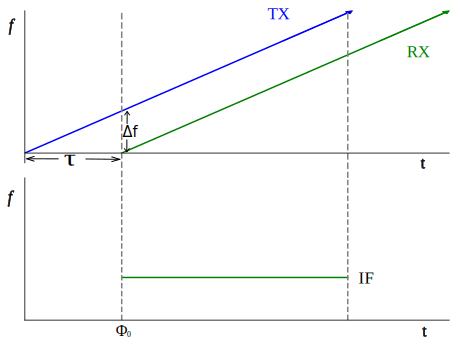
\includegraphics[width=0.6\textwidth]{figures/if1.pdf}\\
	\caption{IF 频率恒定不变}
	\label{IF}
\end{figure}

\begin{equation}
	\tau = \frac{\Delta f}{S}
	\label{tau0}
\end{equation}
通过公式\eqref{tau1}代入$\tau$后可推导出$d$,其中 $d$ 是与被检测物体的距离,$c$ 是光速。
\begin{equation}
	\tau = \frac{2d}{c}
	\label{tau1}
\end{equation}
图\ref{IF}中IF 信号的初始相位$\Phi_0$是IF信号起点对应的时间点,即图\ref{IF}中左侧垂直虚线表示的时间点发送信号相位与接收信号相位之差。
\begin{equation}
	\Phi_0 = 2\pi f_c \tau = \frac{4\pi d}{\lambda}
	\label{phi0}
\end{equation}

\begin{figure}[htbp]
	\centering
	% Requires \usepackage{graphicx}
	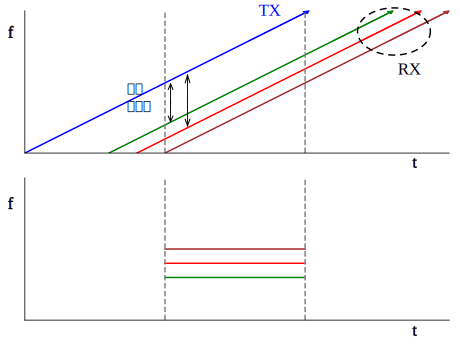
\includegraphics[width=0.6\textwidth]{figures/ifs.pdf}\\
	\caption{多个物体IF信号}
	\label{IFS}
\end{figure}


在检测多个物体的情况下会收到多个物体的反射信号。每个反射信号的延时都不一样,延时与该物体的距离成正比。不同的反射信号转化为多个IF中频信号并混合在一起如图\ref{IFS},每个信号频率恒定。这个包含多个信号的IF信号必须使用傅里叶变换加以处理,以便分离不同的IF中频信号。傅里叶变换处理将会产生一个具有不同的分离峰值的频谱,每个峰值代表对应的距离处存在物体。


\subsection{FMCW雷达测速}
为测量速度,FMCW雷达会周期性地发送Chrip信号,每个Chrip之间存在$T_c$的时间间隔。目标反射的信号通过距离维FFT检测目标的距离。对应于每个线性调频脉冲的距离维FFT将在同一位置出现峰值\cite{rao2017introduction},但相位不同。测得的相位差与速度为$v$的物体在$T_c$间隔的移动对应。相位差可以通过公式\eqref{phi0}推导出公式\eqref{deltaPhi}:
\begin{equation}
	\Delta \Phi = \frac{4\pi V_{T_c}}{\lambda}
	\label{deltaPhi}
\end{equation}
可以通过公式\eqref{v1}推导出速度:
\begin{equation}
	v = \frac{\lambda \Delta \Phi}{4\pi T_c}
	\label{v1}
\end{equation}
由于基于相位差的速度测量仅在$\lvert \Delta \Phi \rvert < \pi $时具有非模糊性\cite{atlas1973doppler},所以使用上述公式可以推断出测速的范围为:
\begin{equation}
	v< \frac{\lambda}{4T_c}
\end{equation}
因此更短的传输间隔可以测量更快的速度。

由离散傅里叶变换\cite{wang1984fast}可知,两个离散的频率$\omega_1$和$\omega_2$在$\omega_1 - \omega_2 > \frac{2\pi}{N}$(N为样本个数)的前提下才可以分辨。因此从公式\eqref{deltaPhi}可知:

\begin{equation}
	\frac{4\pi V_{T_c}}{\lambda} > \frac{2\pi}{N}
\end{equation}
代入帧周期$T_f = N T_c$可得:
\begin{equation}
	v > \frac{\lambda}{2N T_c} = \frac{\lambda}{2 T_f}
\end{equation}
雷达的速度分辨率与帧时间成反比。

% \subsection{CFAR算法} % todo CFAR算法

\section{点云配准相关技术}

\subsection{刚性点云配准算法}
刚性点云配准主要目标是找到两个点云之间的最佳转换\cite{tam2012registration},以使它们在空间中更好地对齐。刚性点云配准是一种在计算机视觉和机器人领域广泛应用的点云配准方法\cite{JSJX201909003}。其基本原理是通过迭代的方式,不断优化两个点云之间的刚体变换使它们的重叠部分最大化。

首先,通过某种方式初始化两个点云的初始对准。可以通过随机设置初始值、粗略的估计、传感器测量或其他方法实现。
通过计算每个点在参考点云中的最近邻点,建立点云之间的初始对应关系。这一步通常使用KD树\cite{bentley1990k}等数据结构来提高匹配效率,KD树的实现算伪代码如算法\ref{alg:kdtree}所示。

\begin{algorithm}[htbp]
	\caption{构建KD树}\label{alg:kdtree}
	\begin{algorithmic}[1]
		\Require 点集$X$,深度$depth$
		\Ensure KD树
		\If{$\text{点集}$ 为空}
		\State \textbf{return} $\text{NULL}$
		\EndIf
		\State $k \gets$ 点的维度
		\State $axis \gets depth \mod k$
		
		\State $P \gets \text{按轴排序}(X, axis)$ \Comment{沿着所选轴对点进行排序}
		
		\State $medianIndex  \gets \text{点集长度} \div 2$ \Comment{获取中值索引}
		
		\State $median \gets P[medianIndex]$ \Comment{获取中值}
		
		\State $node \gets \text{创建节点}(median, axis)$ \Comment{创建一个新的KD树节点}
		
		\State $node.left \gets \text{构建KD树}(P[1 : medianIndex-1], depth + 1)$
		\State $node.right \gets \text{构建KD树}(P[medianIndex+1 : len(P)], depth + 1)$
		
		\State \textbf{return} node
	\end{algorithmic}
\end{algorithm}

利用最近邻匹配得到的对应关系,计算两个点云之间的最佳刚体变换,通常采用最小二乘法等优化算法。在采用最小二乘法计算点云距离的算法中,通过拟合一个模型来估计点云之间的距离。最小二乘法的核心思想是最小化残差平方和,即观测值与模型预测值之间的差异。假设有源点云$P$和参考点云$Q$如公式\eqref{点云表示}所示,其中$P$和$Q$分别表示源点云和参考点云,$p_i$和$q_i$分别表示源点云和参考点云中的点。需要求出变换矩阵$R$和平移变量$t$使得$\forall i, q_i=Rp_i + t$。
\begin{equation}
	\label{点云表示}
	\begin{split}
		P =  \left\lbrace p_1, p_2,\ldots,p_n \right\rbrace\\
		Q =  \left\lbrace q_1, q_2,\ldots,q_n \right\rbrace
	\end{split}
\end{equation}

使用初始的$R_0,t_0$或上一次迭代得到的的$R_k,t_k$ 对初始点云进行变换,得到一个临时变换的点云,然后继续用得到的点云与参考点云进行比较,找出当前源点云中每一个点在参考点云中的最近邻点,基于最小二乘法进行迭代计算,使得误差平方和达到极小值。

\begin{equation}
\label{最小化Rt}
R,t = \mathop{\arg\min}_{R,t}\sum_{i=1}^{n} \|\left( Rp_i+t\right) -q_i \| ^2
\end{equation}


计算最优平移$t$,令 $N=|P|$ ,由公式\eqref{最小化Rt}可知,此时迭代的损失表示为:
\begin{equation}
	\label{损失公式1}
	F(t) = \sum_{i=1}^{N} \| (R\cdot p_i + t) - q_i\|^2
\end{equation}

对损失求偏导可得:
\begin{equation}
	\label{损失公式1偏导}
	\begin{split}
		\frac{\partial F}{\partial t} &= \sum_{i=1}^{N}2(R \cdot p_i + t-q_i)\\
		&=2nt + 2R\sum_{i=1}^{N}p_i -  2R\sum_{i=1}^{N}q_i
	\end{split}
\end{equation}


令$\frac{\partial F}{\partial t} = 0$,可得:
\begin{equation}
	\label{最优平移计算}
	\begin{split}
			t &= \frac{1}{N}\sum_{i=1}^{N} q_i - R\sum_{i=1}^{N}p_i\\
		&= \bar{q} - R\bar{x}
	\end{split}
\end{equation}

由公式\eqref{最优平移计算}可知,loss最小的最优平移可以由最优旋转$R$和两个点云的质心求出。

接下来求最优旋转$R$,由最佳平移的证明过程可知,最优平移由最优旋转通过点云的质心计算得到。为了计算简单,先将点云所有的点以质心为中心平移。即令$\hat{p_i} = p_i - \bar{p}$,$\hat{q_i} = q_i - \bar{q}$。此时loss的形式转变为:

\begin{equation}
	\label{损失公式}
	F(R) = \sum_{i=1}^{N} \| R\cdot\hat{p_i} - \hat{q_i}  \|^2
\end{equation}
先对$ \| R\cdot\hat{p_i} - \hat{q_i}  \|^2$ 进行公式\eqref{eq:绝对值计算}计算:
\begin{equation}
	\label{eq:绝对值计算}
	\begin{split}
		\| R\cdot\hat{p_i} - \hat{q_i}  \|^2 &= ( R\cdot\hat{p_i} - \hat{q_i})^T ( R\cdot\hat{p_i} - \hat{q_i}) \\
		&= ( \hat{p_i}^T \cdot R^T - \hat{q_i}^T) ( R\cdot\hat{p_i} - \hat{q_i}) \\
		&= \hat{p_i}^T \cdot R^T  R\cdot\hat{p_i} -  \hat{p_i}^T \cdot R^T  \hat{q_i} -  \hat{q_i}^TR\cdot\hat{p_i} +  \hat{p_i}^T \hat{q_i} \\
		&= \| \hat{p_i} \| ^2 +  \| \hat{q_i} \| ^2 - -  \hat{p_i}^T \cdot R^T  \hat{q_i} -  \hat{q_i}^TR\cdot\hat{p_i} \\
		&=  \| \hat{p_i} \| ^2 +  \| \hat{q_i} \| ^2  - 2 \hat{q_i}^TR\cdot\hat{p_i}
	\end{split}
\end{equation}
由于$ \| \hat{p_i} \| ^2 +  \| \hat{q_i} \| ^2 $是不变,最小化公式\eqref{损失公式}转化为求$R^{\prime}$:
\begin{equation}
	R^{\prime} = \arg\min_{R} ( - 2\sum_{i=1}^{N} \hat{q_i}^TR\cdot\hat{p_i})
\end{equation}
即求:
\begin{equation}
	R^{\prime} = \arg\max_{R}(\sum_{i=1}^{N}\hat{q_i}^TR\cdot\hat{p_i})
\end{equation}
由矩阵迹的性质可知:
\begin{equation}
\sum_{i=1}^{N}\hat{q_i}^TR\cdot\hat{p_i} = tr(Y^T R P) =  tr(R P Q^T )
\end{equation}
令 $H= PQ^T$,对$H$做SVD分解可得:
\begin{equation}
H=U\Sigma V^T
\end{equation}
原问题转化为使$tr(RH)$最大,$H$可以分解为$H=U\Sigma U^T$,其中$U$是一个正交矩阵,$\Sigma$是对角矩阵,可得:
\begin{equation}
	tr(R X Y^T ) = tr(RH) = tr(RU\Sigma V^T)= tr(\Sigma V^TRU)
\end{equation}
令$M=V^TRU$,$M$是正交阵,列向量$m_{i}$是正交向量,即$m_i^Tm_i=1$,因此$M$的所有元素$m_{ij}<1$。
\begin{equation}
	tr(\Sigma M)
	\begin{pmatrix}
		\sigma_1  &  &   \\
		&\sigma_2   & \\
		&    &\sigma_2 
	\end{pmatrix}
	\begin{pmatrix}
		m_{11}  &m_{12}   &m_{13}  \\
		m_{21}   &m_{22}   &m_{23}  \\
		m_{31}   &m_{32}   &m_{33} 
	\end{pmatrix}
	= \sigma_1 m_{11} + \sigma_2 m_{22} + \sigma_3 m_{33}
\end{equation}
由此可知,只有当$m_{ii} = 1$的时候,$tr(\Sigma M)$最大,又因为$M$为正交阵,所以$M$为单位阵,可得:
\begin{equation}
	V^TRU = I
\end{equation}
\begin{equation}
	R=VU^T
\end{equation}


总结以上计算过程,在已经求出对应点的情况下,设$\bar{x},\bar{y}$分别为$X$点云和$Y$点云的质心,令$\hat{p_i} = p_i - \bar{p}$,$\hat{q_i} = q_i - \bar{q}$,$N=|P|$,$H=\sum_{i=1}^{N}p_iq_i^T$,$H$为$3\times3$的矩阵,对$H$进行SVD分解可得$H=U\Sigma V^T$,其中$U$是一个$m\times m$的矩阵, $U$和$V$都是酉矩阵,$\Sigma$为对角是奇异值的矩阵。则ICP在此次迭代的旋转为:
\begin{equation}
	\label{旋转公式}
R^* = VU^T
\end{equation}
平移为:
\begin{equation}
	\label{平移公式}
t^* = \bar{q} - R^*\bar{p}
\end{equation}

将刚体变换应用于移动的点云,更新点云的位置,然后迭代执行最近邻匹配和刚体变换的步骤,直至收敛或达到预定的迭代次数。


以上步骤如算法\ref{刚性配准}所示。
\begin{algorithm}[htbp]
	\caption{刚性配准}\label{刚性配准}
	\begin{algorithmic}[1]
		\Require $\text{点云}_1$, $\text{点云}_2$
		\Ensure 刚性变换$T$
		\State \text{当前}${R,t} \gets \text{初始化}(\text{点云}_1, \text{点云}_2)$
		
		\While{未收敛}
		\State 寻找最近迭代点
		\State 计算对应关系
		\State ${R,t}$  \gets 计算SVD分解
		\State $\text{点云}_1$ \gets 应用变换$(\text{点云}_1, R,t)$
		\EndWhile
		
		\State $T_{\text{最优}} \gets T_{\text{当前}}$
		\State \textbf{return} $T_{\text{最优}}$
	\end{algorithmic}
\end{algorithm}
\subsection{点云配准的评价指标}
点云配准的评价指标是用于评价配准结果的好坏,常用的指标有:均方误差(Mean Square Error,MSE)、平均绝对误差(Mean Absolute Error,MAE)、均方根误差(Root Mean Square Error,RMSE)等。均方误差是指预测值与真实值之间误差平方的平均值,其公式表示为:
\begin{equation}
	\text{MSE} = \frac{1}{N}\sum_{i=1}^{N}(y_i - \hat{y_i})^2
	\label{MSE}
\end{equation}
其中,$y_i$为真实值,$\hat{y_i}$为预测值。

平均绝对误差是指预测值与真实值之差的绝对值的平均值,其公式表示为:
\begin{equation}
	\text{MAE} = \frac{1}{N}\sum_{i=1}^{N}\|y_i - \hat{y_i} \|
	\label{MAE}
\end{equation}
其中,$y_i$为真实值,$\hat{y_i}$为预测值。

均方根误差是指预测值与真实值之间误差平方根的平均值,其公式表示为:
\begin{equation}
	\text{RMSE} = \sqrt{\frac{1}{N}\sum_{i=1}^{N}(y_i - \hat{y_i})^2}
	\label{RMSE}
\end{equation}
其中,$y_i$为真实值,$\hat{y_i}$为预测值。

\section{深度学习相关理论}

\subsection{残差神经网络} 
残差神经网络(Residual Neural Network,ResNet)是由微软亚洲研究院的研究员何恺明等人提出的一种深度卷积神经网络。ResNet的核心思想是引入了残差学习,通过引入跨层的连接,使得网络可以学习残差,从而解决了深度神经网络训练过程中的梯度消失和梯度爆炸问题。一个典型的残差块如图\ref{ResidualBlock}所示,其中$x$为输入,$F(x)$为残差块的输出,$F(x)$与$x$相加后再通过激活函数得到最终的输出$y$。
\begin{figure}[htbp]
	\centering
	\includegraphics[width=0.5\textwidth]{figures/残差块.pdf}\\
	\caption{残差块}
	\label{ResidualBlock}
\end{figure}
残差神经网络在传统神经网络的基础上,将上一层(L-1层)的输出直接图加到了当前层(L层)的输出上,即:
\begin{equation}
	y = F(x) + X
\end{equation}
此时,L层神经网络所能拟合的函数必然包含了L-1层神经网络所能拟合的函数,因此残差神经网络的深度可以更深,从而可以更好地拟合复杂的函数。

\subsection{自注意力机制}
自注意力机制(Self-Attention Mechanism)是一种用于处理序列数据的机制,它可以在不同位置之间建立长距离的依赖关系,从而更好地捕捉序列数据的全局信息。自注意力机制的核心思想是通过计算序列中不同位置之间的相关性,从而得到每个位置的权重,然后根据这些权重对序列中的每个位置进行加权求和,得到序列最终的表示。自注意力机制的计算过程如图\ref{self-attention}所示,其中$Q,K,V$分别表示查询、键、值,通过计算查询和键的相关性得到权重,然后根据权重对值进行加权求和得到最终的输出。


自注意力机制的计算过程如下:
\begin{equation}
	\text{Attention}(Q,K,V) = \text{softmax}\left(\frac{QK^T}{\sqrt{d_k}}\right)V
\end{equation}
\begin{figure}[htbp]
	\centering
	\includegraphics[width=\linewidth]{figures/注意力.pdf}
	\caption{自注意力机制}
	\label{self-attention}
\end{figure}
\section{本章小结}
本章对FMCW雷达、点云配准和深度学习相关理论技术进行了介绍。首先介绍了FMCW雷达的工作原理和测距、测速的方法,然后介绍了点云配准的基本原理和刚性点云配准的概念,最后介绍了深度学习中的残差神经网络和自注意力机制。以上技术理论为后续的研究工作提供了理论支撑。

\chapter{基于距离多普勒图空间相关性的目标点检测方案}
本章提出了一种基于残差神经网络和十字交叉注意力机制的毫米波雷达距离多普勒图目标点检测方案RA-CFAR,该方案解决了传统CFAR方法设置参数不良可能导致的检测异常,在多目标场景和较低信噪比环境下能够更有效地检测目标点。首先,将毫米波雷达一帧发送的N个Chrip和与收到信号混合成N个中频信号,其次在每个Chrip中提取出M个IF信号样本,然后对距离和多普勒两个维度进行FFT运算生成距离多普勒图,最后使用残差神经网络以及十字交叉注意力模块来处理输入的距离多普勒图,学习图中的空间局部自相关性给出目标点检测的评估值。在本章,将RA-CFAR与CA-CFAR、OS-CFAR等多种算法在公开数据集上进行对比实验,验证了方案的有效性。

\section{距离多普勒图目标点检测概述} \label{距离多普勒图目标点检测问题分析与方案设计}
\subsection{距离多普勒图目标点检测问题分析}

毫米波雷达目标点检测方案的基本原理是根据检测单元的邻近单元评估距离多普勒图中一个单元格周围的噪声水平,并通过设置适当的阈值来检测目标。然而,在低信噪比和多目标场景下,由于目标信号的强度可能会与背景噪声相近,以及多个目标同时出现信号会相互干扰,CFAR算法会因此受到影响导致性能发生退化而无法有效检测目标点。此外传统CFAR算法存在难以设置合理参数的问题,较差的参数设置会导致性能的显著下降。因此,需要一个更加有效的目标点检测方案,这个方案需要在较低信噪比和多目标的场景下有效检测出目标点,并且克服CFAR算法参数难以设置的问题。

\subsection{RA-CFAR距离多普勒图目标点检测方案}

基于上述问题分析,本章采用了由多个残差块组成的残差神经网络和注意力机制,构建了RA-CFAR的网络结构。为提高不同场景下的目标点检测准确度,构建了用于生成不同场景高质量距离多普勒图数据集的生成流程,为后续目标点检测提供多场景数据集支撑。由于距离多普勒图蕴含丰富信息,残差神经网络的跳跃连接有助于信息更有效地在网络中传播,从而促进目标特征的捕捉。此外,考虑到距离多普勒图中目标点的位置差异性,需要模型有效地提取位置信息,引入了十字交叉注意力\cite{huang2019ccnet}模块从横纵两个方向更好地捕捉空间位置的关联性。为有效评估背景噪声水平以及运动目标数量对于目标点检测的影响,使用建立的信号模型根据信噪比水平以及运动目标数量生成指定场景的距离多普勒图。距离多普勒图的处理流程以及目标点检测的流程如图\ref{fig:目标点检测流程}所示。

\begin{figure}[htbp]
	\centering
	\includegraphics[width=\linewidth]{figures/目标点检测流程.pdf}
	\caption{目标点检测流程}
	\label{fig:目标点检测流程}
\end{figure}


\section{多场景距离多普勒图数据集构建}

\subsection{数据预处理}
一帧的雷达数据含有N个Chrip信号,首先要做的是对每个Chrip做FFT运算,这一步的FFT运算将雷达的回波信号分离成不同距离门限的信号,处理一帧中N个Chrip的信号,并且将得到的频谱以列的方式存储到二维矩阵中。接下来对于每个距离门限的行进行长度为N的FFT运算,测量雷达目标的多普勒频率。经过两次FFT运算得到了一帧距离多普勒图。过程如图\ref{fig:FFT运算}所示。
\begin{figure}[htbp]
	\centering
	\includegraphics[width=0.8\linewidth]{figures/FFT运算.pdf}
	\caption{FFT运算}
	\label{fig:FFT运算}
\end{figure}


经过二维FFT处理得到的距离多普勒图中存在两种主要类型的干扰:直流分量和静态干扰。直流分量通常是由雷达系统中的直流偏置引起的\cite{gu2000removal},表现为频域中的零频分量。这些直流偏置是由雷达系统中的一些器件,例如放大器和混频器引起的,它们可能会对雷达信号的处理和分析产生影响,从而影响后续的特征提取和分类过程。静态干扰是由场景中静态物体引起的,它在距离多普勒图中表现为速度为0m/s的区域。

除了干扰峰值外,还存在一些峰值与干扰峰值不同,这些峰值对应于移动目标的速度信息。根据多普勒效应,当一个物体相对于雷达运动时,回波信号的频率会发生变化,在速度维上产生频移。通过执行速度维FFT,能够将回波信号在速度维上展开,得到不同速度的目标信息。在距离多普勒图中静态干扰位于速度零轴附近,移动目标对应的峰值位于速度轴两侧。根据峰值的位置能够确定目标的速度方向,峰值的幅度大小反映了目标的速度强度。在噪声和干扰峰值中检测出有效的目标点是毫米波雷达目标点检测的关键问题。
为了获取准确的训练集和测试集,本章使用仿真的方式模仿FMCW雷达发射信号和接受信号的过程,通过建立线性调频连续波模型,发送频率随时间线性变化的波形,模拟FMCW雷达的工作,在收到的回波信号里面加入控制信噪比的高斯噪声。
本章的实验环境如表\ref{实验软硬件环境}所示:

% \begin{table}[htbp]
%     \centering
% 	\caption{实验软硬件环境}
% 	\begin{tblr}{
% 		hline{1,Z} = {1pt},
% 		hline{2},
% 		colspec={cc},
% 	}
% 		软件环境  & 硬件环境 \\
% 		系统:Windows 11   & CPU Intel i7-11700 \\
% 		语言:Python 3.9 MATLAB R2023b    & 内存32G \\
% 		Cuda 11.1 Pytorch 1.10.1   & 硬盘1TB \\
% 		采集工具:mWave Studio   & IWR6843 DCA1000EVM \\
% 	\end{tblr}
% 	\label{实验软硬件环境}
% \end{table}     

\begin{table}[htbp]
	\centering
	\tabcolsep=1cm
	\caption{实验软硬件环境}
	\begin{tabular}{cc}
		\toprule
		软件环境  & 硬件环境 \\
		\midrule
		系统:Windows 11   & CPU Intel i7-11700 \\
		语言:Python 3.9 MATLAB R2023b    & 内存32G \\
		Cuda 11.1 Pytorch 1.10.1   & 硬盘1TB \\
		采集工具:mWave Studio   & IWR6843 DCA1000EVM \\
		\bottomrule
	\end{tabular}
	\label{实验软硬件环境}
\end{table}

\subsection{信号模型建立} \label{信号模型建立}
因为FMCW雷达发射信号的频率是一个随时间变化的线性函数,如图\ref{chrip}所示。发送信号的模型\cite{DBLP:journals/tcas/GerstmairMOSH18}可以使用公式\eqref{eq:发送信号}表示。公式中$signal(t)$为当前发射的信号,$A$为信号的幅度,$S$为Chrip信号随时间线性变化的斜率,$T$为当前帧的周期,$f_0$为载频。
\begin{equation}
	\label{eq:发送信号}
	S_t(t) = A \cos\big(2\pi (f_0t+\frac{St^2}{2}) + \phi_0 \big), t \in [0,T]
\end{equation}
由此可得,FMCW雷达发送信号模型的相位可以用公式\eqref{eq:发送相位}表示:
\begin{equation}
	\label{eq:发送相位}
	P_t(t) = 2\pi (f_0t+\frac{St^2}{2})+ \phi_0, t \in [0,T]
\end{equation}
经过每个时间间隔$\tau$,都会发送一个Chrip信号。利用多个Chirp来测量目标的速度。

\begin{figure}[htbp]
	\centering
	\subcaptionbox{幅度变化}{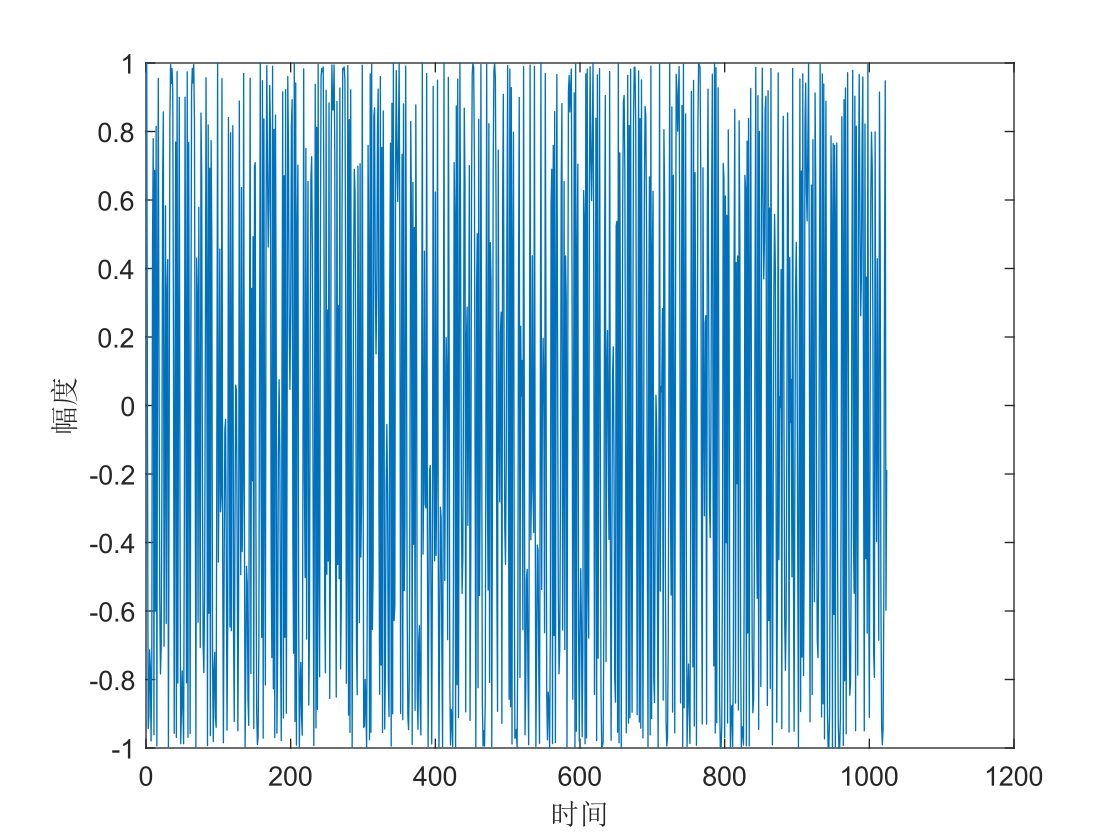
\includegraphics[width = 0.45\textwidth]{figures/发射信号幅度.pdf}}
	\subcaptionbox{频率变化}{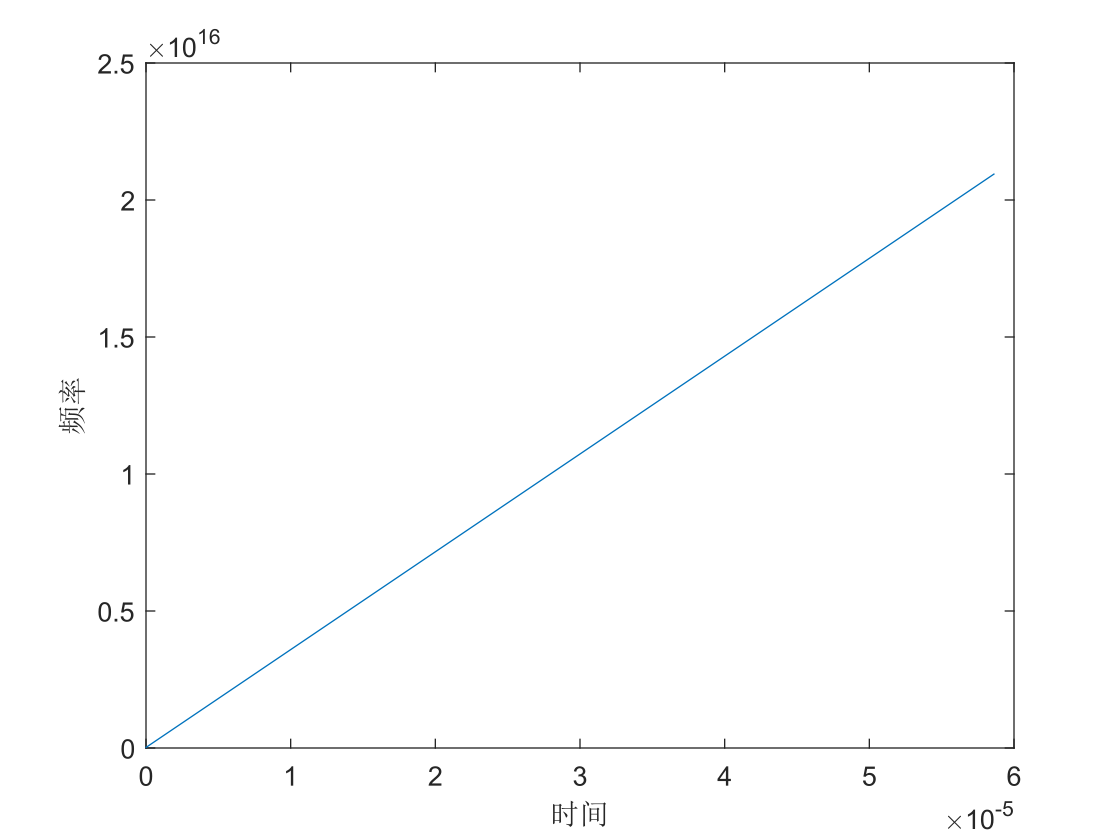
\includegraphics[width = 0.45\textwidth]{figures/发射信号频率.pdf}}
	\caption{发送信号时频域图}
	\label{fig:发送信号时频域图}
\end{figure}

已知电磁波的传输速度为光速$c$,假设测量目标与雷达的距离为$R$,则雷达收到回波信号的延迟为$\tau=\frac{2R}{c}$,$K$为雷达接收到信号的衰减系数\cite{matrosov2008assessment}。因此由公式\eqref{eq:发送信号}可知,接收到的回波信号的模型如公式\eqref{eq:接受信号}所示:
\begin{equation}
	\label{eq:接受信号}
	S_r(t) = KA \cos\big(2\pi (f_0(t - \tau)+\frac{S(t-\tau)^2}{2}) + \phi_0 \big), t \in [0,T]
\end{equation}
由公式\eqref{eq:发送相位}和\eqref{eq:接受信号}可得,回波信号的相位模型为:
\begin{equation}
	\label{eq:接收相位}
	P_r(t) = 2\pi \big(f_0(t-\tau)+\frac{S(t-\tau)^2}{2}\big)+ \phi_0, t\in [0,T]
\end{equation}
将接收到的回波信号$S_r(t)$与发送信号$S_t(t)$进行混频后,经过低通滤波就可以得到一个差频信号,这个信号是单一频率的正弦波。差频信号的相位表达式如下:
\begin{equation}
	\label{eq:中频}
	\begin{split}
		P_t(t) - P_r(t) &= \Big(2\pi(f_0t+\frac{St^2}{2})+\phi_0\Big) - \Big(2\pi \big(f_0(t-\tau)+\frac{S(t-\tau)^2}{2}\big)+ \phi_0\Big) , t\in [0,T]\\
		&=2\pi f_0\tau + 2\pi S \tau t - \pi S \tau^2
	\end{split}
\end{equation}
为了模拟真实的场景,需要在回波信号中添加指定信噪比(Signal to Noise Ratio,SNR)的高斯噪声\cite{luisier2010image}。回波信号的模型函数公式\eqref{eq:接受信号}是已知的,在已知原始干净信号后,SNR的计算公式如\eqref{eq:SNR}所示:
\begin{equation}
	\label{eq:SNR}
	SNR = 10\log10(signalPower / Power(noisedSignal- Signal))
\end{equation}

因此添加一个已知SNR的噪声步骤如下:
\par
(1)计算原始信号的平均功率:
\begin{equation}
	signalPower = sum(abs(S_r)^2) / length(S_r)
\end{equation}

(2)将平均功率转为dB:
\begin{equation}
	signalPowerdB = 10\log10(signalPower)
\end{equation}
\par
(3)计算噪声的平均功率(dB):
\begin{equation}
	noisePowerdB = signalPowerdB -SNR
\end{equation}
\par
(4)计算噪声的平均功率:
\begin{equation}
noisePower = 10^{(noisePowerdB /10)}
\end{equation}
\par
(5)最后得到需要添加的噪声为:
\begin{equation}
noise = \sqrt{noisePower}*randn(length(S_r),1)
\end{equation}
\subsection{训练数据生成} \label{训练数据生成}
为了得到与距离多普勒图目标点对应的真实标签值,本节采用仿真环境建立数据集。由于不同的噪声水平和目标数量会影响到特征提取的成功率,为了提高模型的泛化能力,本节根据不同动目标速度生成回波信号并且根据不同的SNR生成并添加噪声,使用添加噪声后的混合信号成距离多普勒图。使用距离多普勒图作为输入数据,动目标图作为标签生成训练数据。
单目标距离多普勒图如图\ref{fig:单目标距离多普勒图}所示,多目标距离多普勒图如图\ref{fig:多目标距离多普勒图}所示。

仿真环境的参数设置如表\ref{仿真环境参数}所示,其中SNR的取值涵盖了从低信噪比到高信噪比的范围,动目标速度为从20-60m/s随机生成。
\begin{figure}[htbp]
	\centering
	\subcaptionbox{距离多普勒}{\includegraphics[width = 0.4\textwidth]{figures/1目标距离多普勒.pdf}}
	\subcaptionbox{动目标图}{\includegraphics[width = 0.4\textwidth]{figures/1目标CFAR.pdf}}
	\caption{单目标距离多普勒图}
	\label{fig:单目标距离多普勒图}
\end{figure}
\begin{figure}[htbp]
	\centering
	\subcaptionbox{二目标距离多普勒}{\includegraphics[width = 0.4\textwidth]{figures/2目标距离多普勒.pdf}}
	\subcaptionbox{三目标动目标图}{\includegraphics[width = 0.4\textwidth]{figures/2目标CFAR.pdf}}
	\subcaptionbox{三目标距离多普勒}{\includegraphics[width = 0.4\textwidth]{figures/3目标距离多普勒.pdf}}
	\subcaptionbox{三目标动目标图}{\includegraphics[width = 0.4\textwidth]{figures/3目标CFAR.pdf}}
	\caption{多目标距离多普勒图}
	\label{fig:多目标距离多普勒图}
\end{figure}

\begin{table}[htbp]
	\centering
	\caption{仿真环境参数}
	\begin{tabular}{cccc}
		\toprule
		\diagbox{SNR}{动目标数量} & 1 & 2 & 3 \\
		\midrule
		20dB & 20dB,1目标& 20dB,2目标& 20dB,3目标\\
		25dB & 25dB,1目标& 25dB,2目标& 25dB,3目标\\
		30dB & 30dB,1目标& 30dB,2目标& 30dB,3目标\\
		35dB & 35dB,1目标& 35dB,2目标& 35dB,3目标\\
		\bottomrule
	\end{tabular}
	\label{仿真环境参数}
\end{table}
\begin{table}[htbp]
	\centering
	\tabcolsep=1cm
	\caption{雷达参数表}
	\begin{tabular}{cc}
		\toprule
		参数 & 数值 \\
		\midrule
		发射天线 & 4  \\
		接收天线 &3   \\
		ADC采样点数 & 128  \\
		开始频率 & 60GHz   \\
		空闲时间 & 10ns  \\
		每帧Chrip数 & 128 \\
		\bottomrule
	\end{tabular}
	\label{雷达参数表}
\end{table}

\subsection{实验数据采集} \label{实验数据采集}
为了验证在实际环境中效果,使用德州仪器IWR-6843毫米波雷达采集了多个环境中的数据。
搭建的实验环境为,使用DCA1000EVM数据采集板通过网口将ADC采样的RAW数据传输到PC上。数据收集的场地为开阔室内和走廊,雷达高度为1.5m。雷达参数配置如表所示,雷达设备如图\ref{fig:实验设备}所示。

\begin{figure}[htbp]
	\centering
	\subcaptionbox{正面}{\includegraphics[width = 0.4\textwidth]{images/正面.jpg}}
	\subcaptionbox{背面}{\includegraphics[width = 0.4\textwidth]{images/背面.jpg}}
	\caption{IWR6843毫米波雷达}
	\label{fig:实验设备}
\end{figure}


每个地点不同的人数采集100组数据,共计采集6000组数据。经过FFT后得到的距离多普勒图大小为$96 \times 128$,室内与室外数据采集参数如表\ref{采集数据参数}所示。
\begin{table}[htbp]
	\caption{采集数据参数}
	\begin{subtable}{.4\linewidth}
		\centering
		\caption{单人采集数据}
		\begin{tabular}{ccc}
			\toprule
		    人员 & 移动速度 & 样本数量  \\
			\midrule
			1号 &2 m/s & 100 \\
			2号 &1 m/s & 100 \\
			3号 &3 m/s & 100  \\
			\bottomrule
		\end{tabular}
	\end{subtable}
	\begin{subtable}{.4\linewidth}
		\centering
		\caption{多人采集数据}
		\begin{tabular}{ccc}
			\toprule
			人数 & 移动速度 & 样本数量  \\
			\midrule
			2人 & 1 m/s,2 m/s& 100 \\
			3人 & 1 m/s,2 m/s,3 m/s & 100  \\
			\bottomrule
		\end{tabular}
	\end{subtable}
	\label{采集数据参数}
\end{table}

\section{距离多普勒图目标点检测方案}

\subsection{基于残差网络的全图特征提取}
残差块模型设计如图\ref{fig:ResidualNet}所示,在每个残差块中,使用二维卷积提取特征,使用$3\times3$的卷积核提取距离多普勒图中的空间局部相关性。网络由四个残差块组成,在残差块后接展平层和两层线性层。

(1)残差块设计。每个残差块包含两个$3\times3$卷积层,两个Batch Norm层,两个Relu层和一个$1\times1$的卷积层用于从输入到输出的跳跃连接。
\begin{figure}[htbp]
	\centering
	\includegraphics[width=\linewidth]{figures/残差网络.pdf}
	\caption{残差网络模型设计}
	\label{fig:ResidualNet}
\end{figure}
当前输入的特征$X$的维度为$(B,1,H,W)$,其中$B$为Batch大小,1为特征通道数,$H$和$W$为输入距离多普勒图的长和宽。输入特征经过两次卷积和两次归一化后,特征$Y$维度变为$(B,64,H,W)$,为了保证网络加深后输入特征不丢失,在残差块输出之前加入原始输入数据。因此时$X$的维度与$Y$的维度不匹配,所以需要$1\times1$的卷积层,将$X$的维度变为$(B,64,H,W)$。残差块输出的$Y=Y+X$。残差块的设置如表\ref{残差块参数设置}所示。

\begin{table}[htbp]
	\centering
	\tabcolsep=3mm
	\caption{残差网络参数设置}
	\begin{tabular}{ccccccc}
		\toprule
		层  & 核大小 & 输入通道 & 输出通道 & 步数 & 填充 & 输出 \\
		\midrule
		Conv & 3 \times 3 & -- & -- & -- & -- & -- \\
		ResidualBlock &3 \times 3 & 1 & 16 & 1 & 1 & B $\times$ 16 $\times$ H $\times$ W \\
		ResidualBlock &3 \times 3 & 16 & 32 & 1 & 1 & B $\times$ 32 $\times$ H $\times$ W \\
		ResidualBlock &3 \times 3 & 32 & 8 & 1 & 1 & B $\times$ 8 $\times$ H $\times$ W \\
		ResidualBlock &3 \times 3 & 8 & 1 & 1 & 1 & B $\times$ 1 $\times$ H $\times$ W \\
		Criss-Cross Attention & -- & 1 & 1 & -- & -- & B $\times$ 8 $\times$ H $\times$ W \\
		Skip Conn & 1 \times 1 & in & out & -- & -- & B $\times$ out $\times$ H $\times$ W \\
		Flatten & -- & -- & -- & -- & -- & B \times (H $\times$ W) \\
		FC & -- &  (H $\times$ W) & 256  & -- & -- & B \times 256 \\
		FC & -- &  256 & 512  & -- & -- & B \times 512 \\
		FC & -- & 512 & (H $\times$ W)  & -- & -- & B \times (H $\times$ W) \\
		\bottomrule
	\end{tabular}
	\label{残差块参数设置}
\end{table}

(2)模型网络设计。RA-CFAR采用了改造后的残差块做为基础,搭建了神经网络模型。使用四个残差块叠加对特征先升维后降维的方式实现距离多普勒图中噪声特征的提取。实验中对比使用五个残差块将特征维度升到64维后降维的方案,训练时间大幅增加而精确度无明显提升,因此采用四个残差块叠加。每个残差块的卷积层之后都使用了批归一化层和Relu层用来缓解网络梯消失的问题,残差块的卷积层中使用$3\times3$的卷积核大小避免丢失距离多普勒图中小范围特征。为减少空间信息的丢失,残差块中的卷积层在提升特征通道数后保留了原图尺寸。为使每个残差块输入与输出维度匹配,使用$1\times1$的卷积核匹配输入输出维度。在残差块之后使用自适应池化层在后两个维度上进行池化。池化之后使用展平层将特征数据展平为一维向量,输入到二层全连接层得到最终的输出结果。

\subsection{基于十字交叉注意力机制的目标点检测}
为了捕捉距离多普勒图中目标点区域的空间位置的关联性,在残差网络模块之后引入十字交叉注意力机制检测目标点。从距离多普勒图中识别目标的任务近似于从图像中分离出目标与背景的任务。注意力机制可以改善目标检测任务中对目标区域的定位和识别能力。通过在图像中的不同位置计算注意力权重,模型可以更好地理解目标与背景之间的关系,并且更准确地定位和识别目标。由于距离多普勒图是从距离维和多普勒维两次FFT运算得到,其目标点单元所在行和列的幅度水平反应了目标点的位置信息。因此,引入十字交叉注意力机制在每个单元的行和列上进行自注意力计算,有效评估目标点的位置信息。

在残差神经网络之后引入十字交叉注意力机制的工作过程分为如下几个步骤:
\par
(1)将残差神经网络提取得到的特征图中每个单元格所在的行和列分别作为自注意力机制的输入,构建查询、键和数值的表示。在经过残差块的特征提取后,获取的特征是与原输入距离多普勒图尺寸相同的但是被展平成一维的特征向量,记此向量为$D$,将其经过$1\times1$卷积后作为自注意力机制特征向量。表示为:
\begin{equation}
	Q=Conv(D)
\end{equation}
其中$Q$是根据输入特征构建的查询向量。通过计算输入查询向量与键值向量的相关性得到输出向量。
\par
(2)获取每个单元格的归一化权重。取$Q$中一单元格的特征通道值$q=Q(i,j)$,$Q$的尺寸为$(1,H,W)$,$H$和$W$分别为距离多普勒图的高和宽,$i$和$j$分别为单元格的行和列。取$K$中与$q$同行和列的所有单元格的特征通道值$k$,交叉位置只取一次。得到$k$的尺寸为$(1,H+W-1)$。将$q$与$k$的特征通道值进行点积运算得到注意力权重$q_{att}$,再对$(H+W-1)$个值进行Softmax操作,得到归一化权重。对$Q$所有单元格进行相同操作,得到所有单元格的归一化权重。得到$A$的尺寸为$(H,W,H+W-1)$。

\par
(3)加权求和。取A中一单元格位置的归一化权重$a=A(i,j)$, $a$的尺寸为$(1, H+W-1)$。将$a$与$V$中同行同列的值进行加权求和,得到输出向量$o$。对$A$中所有单元格进行相同操作,得到所有单元格的输出向量。得到$o$的尺寸为$(1,H,W)$。输出向量计算如公式\eqref{eq:加权求和}所示。
\begin{equation}
	\label{eq:加权求和}
	o = \sum_{i=1}^{H+W-1}a_i v_i
\end{equation}
其中$v_i \in V$表示注意力机制中的值向量,在本节中为经过残差神经网络提取后的特征值。通过加权计算得到的特征$o$反应了$i,j$位置与其他位置的空间相关性。十字交叉注意力机制的工作流程如图\ref{fig:十字交叉注意力机制}所示。
\begin{figure}[htbp]
	\centering
	\includegraphics[width=0.7\linewidth]{figures/十字交叉注意力机制.pdf}
	\caption{十字交叉注意力机制}
	\label{fig:十字交叉注意力机制}
\end{figure}


将注意力模块加入到网络后,整体网络模型如图\ref{fig:整体网络}所示。
\begin{figure}[htbp]
	\centering
	\includegraphics[width=\linewidth]{figures/整体网络.pdf}
	\caption{整体网络模型设计}
	\label{fig:整体网络}
\end{figure}

\subsection{训练流程}
(1)损失函数设计。本方案的输出结果为距离多普勒图中每一个单元是否有目标存在,可以抽象为对每个单元进行二分类问题。将单元格的输出视为概率,对每个单元格的输出结果与标签值,使用交叉熵损失函数用来衡量两个概率分布之间的距离。交叉熵损失函数的表达式如下:
\begin{equation}
	\label{eq:交叉熵损失函数}
	L(y,\hat{y}) = -\frac{1}{N}\sum_{i=1}^{N}y_i\log(\hat{y}_i) + (1-y_i)\log(1-\hat{y}_i)
\end{equation}
其中$y$为真实标签,$\hat{y}$为预测标签,$N$为样本数量。交叉熵损失函数的值越小,模型的预测结果越接近真实标签。

(2)优化器设计。在训练过程中,使用Adam优化器作为优化器。Adam优化器是一种自适应学习率的优化器,它可以根据每个参数的梯度自适应地调整学习率。Adam优化器的更新公式如\eqref{eq:Adam优化器}:
\begin{equation}
	\label{eq:Adam优化器}
	\begin{split}
		m_t &= \beta_1m_{t-1}+(1-\beta_1)g_t \\
		v_t &= \beta_2v_{t-1}+(1-\beta_2)g_t^2 \\
		\hat{m}_t &= \frac{m_t}{1-\beta_1^t} \\
		\hat{v}_t &= \frac{v_t}{1-\beta_2^t} \\
		\theta_{t+1} &= \theta_t - \frac{\alpha}{\sqrt{\hat{v}_t}+\epsilon}\hat{m}_t
	\end{split}
\end{equation}
其中$\beta_1$和$\beta_2$分别是梯度的一阶矩估计和二阶矩估计的指数衰减率,$\alpha$是学习率,$\epsilon$是为了数值稳定性而添加的小常数。

(3)训练过程中模型性能评估方式。在训练过程中不能直接只以准确率作为评价模型当前性能的指标,由于在距离多普勒图中,无目标点单元和有目标点单元分布不均匀,目标点单元占90\%以上,在判断时即使将所有的点判定为无目标,精确度也为90\%以上。为了正确评估训练过程中模型的性能,在本节除了准确率外还引入了精确率(Precission)、召回率(Recall),F1值作为性能评估指标\cite{goutte2005probabilistic}。目标点检测结果的分类如下:
\par TP(True Positive):真正例,有目标点单元检测为有目标点;
\par TN(True Negative):真反例,无目标点单元检测为无目标点;
\par FP(False Positive):假正例,无目标点单元检测为有目标点;
\par FN(False Positive):假反例,有目标点单元检测为无目标点。
\par 
精确率的含义为在模型检测出的有目标点数量占所有检测为有目标点数量的百分比,计算公式如下:
\begin{equation}
	\label{eq:精确率}
	Precision = \frac{TP}{TP+FP}
\end{equation}
召回率的含义为模型检测出的有目标点数量占所有目标点数量的百分比,计算公式如下:
\begin{equation}
	\label{eq:召回率}
	Recall = \frac{TP}{TP+FN}
\end{equation}
F1值是精确率和召回率的调和平均数,为了能够综合评价模型的性能,计算公式如下:
\begin{equation}
	\label{eq:F1值}
	F1 = \frac{2 \times Precision \times Recall}{Precision + Recall}
\end{equation}

(4)训练过程。使用交叉熵损失函数作为损失函数\cite{4767189},使用Adam优化器作为优化器,学习率为0.0001,批大小为8,训练的epoch数量为30。训练过程中将训练集分为训练集和验证集,训练集用来训练模型,验证集用来评估模型的性能。在每个epoch结束后,在验证集上评估模型的性能,使用Early Stopping策略\cite{yao2007early},当模型的性能没有提升时提前结束训练。训练过程中使用学习率衰减策略,当模型的性能没有提升时减小学习率。训率过程中的准确率、精确率、召回率、F1值曲线如图\ref{fig:RA-CFAR训练曲线}所示。

\begin{figure}[htbp]
	\centering
	\subcaptionbox{准确率(Accuracy)}{\includegraphics[width = 0.48\linewidth]{figures/准确率.pdf}}
	\subcaptionbox{精确率(Precision)}{\includegraphics[width = 0.48\linewidth]{figures/精确率.pdf}}
	\subcaptionbox{召回率(Recall)}{\includegraphics[width = 0.48\linewidth]{figures/召回率.pdf}}
	\subcaptionbox{F1值}{\includegraphics[width = 0.48\linewidth]{figures/F1值.pdf}}
	\caption{RA-CFAR训练曲线}
	\label{fig:RA-CFAR训练曲线}
\end{figure}


\section{实验设计与结果分析}
本节将RA-CFAR与其他几种常用的CFAR算法进行对比,通过对比实验结果分析RA-CFAR的性能。实验数据集为仿真数据集和实际采集的数据集。仿真数据集以\ref{训练数据生成}中同样的方式生成,采集数据集为\ref{实验数据采集}中数据集。实验评估指标为虚警率-检测率曲线和信噪比-检测率曲线。
\subsection{实验评估指标}
为了准确评估R-CFRA的性能,采用虚警率-检测率曲线在不同的信噪比下评估算法的性能。虚警率是指将背景噪声错误识别为目标的概率,检测率是正确识别目标点的比例。

对于输入的信号,可以用目标存在$H_0$和目标不存在$H_1$两个假设。假设$Z$为背景噪声的水平估计,$T$为参考门限因子,则$T \times Z$为门限值,当检测值$Y > T \times Z$,可以认为发现目标,反之没有目标。虚警率是在$H_0$的前提下,检测到目标。即可以表示为
$P(Y>TZ|H_0)$
由于噪声或杂波经过平方检波器后为指数分布,参考单元的概率密度函数为:
\begin{equation}
	f(x)=\frac{1}{2\mu}e^{-\frac{x}{2\mu}},x \ge 0
\end{equation}
从而得到虚警率的计算公式为:
\begin{equation}
	\begin{split}
			P_{fa} &= E \big( P(Y>TZ|H_0) \big) \\
			&= E_Z\big( \int_{T Z}^{\infty} f(y) d y \big)\\
			&= E_Z\big( \int_{T Z}^{\infty} \frac{1}{2\mu}e^{-\frac{y}{2\mu}} d y  \big)\\
			&= E_Z \big( e^{-\frac{TZ}{2\mu}} \big) \\
	\end{split}	
	\label{虚警率公式}
\end{equation}
\subsection{实验算法对比}
本节介绍了其他几种常用的CFAR算法,通过对比其他算法的表现分析算法性能。对比算法有CA-FAR、GOCA-CFAR、SOCA-CFAR、OS-CFAR。
\par
(1)CA-CFAR的背景杂波噪声计算公式是检测单元前后$N$个单元的平均值。
\begin{equation}
	Z_{CZ} = \frac{1}{N}\sum_{i=1}^{N}X_i
\end{equation}
计算门限因子的公式为:
\begin{equation}
	T_{CZ} = N(P^{\frac{1}{N}} - 1)
\end{equation}
\par
(2)GOCA-CFAR是选取检测单元前n个参考单元之和平均值与后n个参考单元之和平均值中大的作为背景杂波噪声评估水平。
\begin{equation}
	\begin{split}
		Y_1 &= \frac{1}{N} \sum_{n}^{i=1}X_i \\
		Y_2 &= \frac{1}{N} \sum_{2n}^{i=n+1}X_i\\
		Z_{GO} &= max\left(Y_1, Y_2\right)
	\end{split}
\end{equation}
计算门限因子需要使用递归方式,公式为:
\begin{equation}
	\begin{split}
	\frac{P_fa}{2} &= \left(1+\frac{T_{GO}}{n} \right)^{-n} -   \left(2+\frac{T_{GO}}{n} \right)^{-n} 
	\cdot  \left\{ \sum_{i=0}^{n-1}\begin{pmatrix}  n+i-1\\i \end{pmatrix} \left(2+ \frac{T_{GO}}{n} \right)^{-k} \right\} \\
	P_fa &= 2\left( 1+T \right)^{-n} -  2\sum_{i=0}^{n-1}\begin{pmatrix}  n+i-1\\i \end{pmatrix}  \left(2+T_{GO} \right)^{-(n+i)}
	\end{split}
\end{equation}
\par
(3)SOCA-CFAR是选取检测单元前n个参考单元之和平均值与后n个参考单元之和平均值中小的作为背景杂波噪声评估水平。
\begin{equation}
	\begin{split}
		Y_1 &= \frac{1}{N} \sum_{n}^{i=1}X_i \\
		Y_2 &= \frac{1}{N} \sum_{2n}^{i=n+1}X_i\\
		Z_{GO} &= min\left(Y_1, Y_2\right)
	\end{split}
\end{equation}
计算门限因子需要使用递归方式,公式为:
\begin{equation}
	\begin{split}
		\frac{P_fa}{2} &=  \left(2+\frac{T_{GO}}{n} \right)^{-n} 
		\cdot  \left\{ \sum_{i=0}^{n-1}\begin{pmatrix}  n+i-1\\i \end{pmatrix} \left(2+ \frac{T_{GO}}{n} \right)^{-k} \right\} \\
		P_fa &= 2\sum_{i=0}^{n-1}\begin{pmatrix}  n+i-1\\i \end{pmatrix}  \left(2+T_{GO} \right)^{-(n+i)}
	\end{split}
\end{equation}
\par
(4)OS-CFAR是先将检测单元排序,选取第$k$个样本作为背景杂波评估水平。
\begin{equation}
	\begin{split}
		Y_1 &= \frac{1}{N} \sum_{n}^{i=1}X_i \\
		Y_2 &= \frac{1}{N} \sum_{2n}^{i=n+1}X_i\\
		Z_{GO} &= min\left(Y_1, Y_2\right)
	\end{split}
\end{equation}
可以使用递归方式计算门限因子,公式为:
\begin{equation}
	P_fa = k \begin{pmatrix}  2n \\k \end{pmatrix} \frac{\left( k-1\right)! \left(T_{OS} + 2n-k \right)! }{\left( T_{OS} + 2n \right)!}
\end{equation}
\par

\subsection{结果分析}
通过比较本章提出RA-CFAR和其他四种CFAR算法的表现,进行实验效果的评估。
\par
(1) 在不同信噪比(本节选择20、25、30、35dB)目标数量(1到3)均匀分布,各个算法检测率随虚警率变化如图\ref{fig:多个SNR检测率}所示。在多个信噪比下,RA-CFAR的虚警率-检测率曲线均优于其他方案。
\begin{figure}[htbp]
	\centering
	\subcaptionbox{SNR=20dB}{\includegraphics[width = 0.48\linewidth]{figures/20_snr.pdf}}
	\subcaptionbox{SNR=25dB}{\includegraphics[width = 0.48\linewidth]{figures/25_snr.pdf}}
	\subcaptionbox{SNR=30dB}{\includegraphics[width = 0.48\linewidth]{figures/30_snr.pdf}}
	\subcaptionbox{SNR=35dB}{\includegraphics[width = 0.48\linewidth]{figures/35_snr.pdf}}
	\caption{多个信噪比下检测率}
	\label{fig:多个SNR检测率}
\end{figure}
\par
为了直观体现性能对比,计算出每条虚警率-检测率曲线下的面积(Area Under Curve,AUC),在各个信噪比下AUC值如表\ref{多信噪比AUC}所示,RA-CFAR在多数情况下取得了良好的效果,在低信噪比的情况下(20dB)相比于其他四种算法AUC值分别提升了4\%、8\%、11.9\%、29.4\%。在信噪比较高的情况下检测效果也与CA-CFAR相当。对比AUC值RA-CFAR在20、25、30dB的情况下均取得了最好的成绩,而在35dB的情况下效果仅次于CA-CFAR,其原因可能是在高信噪比的情况下目标与背景之间的差异更加显著,从而使得目标检测更容易。
\begin{table}[htbp]
	\centering
	\tabcolsep=2mm
	\caption{多信噪比AUC}
	\begin{tabular}{cccccc}
		\toprule
		噪声 & CA-CFAR  & SOCA-CFAR & GOCA-CFAR&OS-CFAR& \textbf{RA-CFAR} \\
		\midrule
		20dB & 0.852 & 0.815 & 0.792 & 0.685 & \textbf{0.887}\\
		25dB & 0.941 & 0.938 & 0.927 & 0.863 & \textbf{0.985} \\
		30dB & 0.980 & 0.973 & 0.975 & 0.966 & \textbf{0.986}\\
		35dB & \textbf{0.987} & 0.979 & 0.980 & 0.975 & 0.986\\
		\bottomrule
	\end{tabular}
	\label{多信噪比AUC}
\end{table}


(2)在相同的虚警率下,检测率随信噪比变化。如图\ref{fig:检测率随信噪比变化}
\begin{figure}[htbp]
	\centering
	\includegraphics[width = 0.6\linewidth]{figures/检测率随信噪比变化.pdf}
	\caption{检测率随信噪比变化}
	\label{fig:检测率随信噪比变化}
\end{figure}
可以看出随着信噪比的增大使目标检测难度变小,所有的算法检测率表现都在变好,但是在低信噪比的情况下RA-CFAR具有明显的优势,当信噪比逐渐增大时RA-CFAR的效果仍优于其他算法。

\begin{figure}[htbp]
	\centering
	\subcaptionbox{SNR=25dB,1目标}{\includegraphics[width = 0.45\textwidth]{figures/1目标.pdf}}
	\subcaptionbox{SNR=25dB,2目标}{\includegraphics[width = 0.45\textwidth]{figures/2目标.pdf}}
	\subcaptionbox{SNR=25dB,3目标}{\includegraphics[width = 0.45\textwidth]{figures/3目标.pdf}}

	\caption{不同目标数量检测率对比}
	\label{fig:不同目标数量检测率对比}
\end{figure}
\begin{table}[htbp]
	\centering
	\tabcolsep=2mm
	\caption{多目标数量AUC}
	\begin{tabular}{cccccc}
		\toprule
		目标数 & CA-CFAR  & SOCA-CFAR & GOCA-CFAR&OS-CFAR& \textbf{RA-CFAR} \\
		\midrule
		1 & 0.978 & 0.976 & 0.973 & 0.973 & \textbf{0.985}\\
		2 & 0.965 & 0.959 & 0.954 & 0.921 & \textbf{0.985} \\
		3 & 0.961 & 0.957 & 0.951 & 0.917 & \textbf{0.983}\\
		\bottomrule
	\end{tabular}
	\label{多目标数量AUC}
\end{table}


(3)在相同的信噪比下,不同目标数量检测率随虚警率变化。为了比较各个算法在不同目标数量时的性能,在本节将SNR固定为25dB,检测各个算法在25dB下不同人数的检测率随虚警率变化。由图\ref{fig:不同目标数量检测率对比}可知,当多目标时其他算法的检测率都出现明显的下降,只有RA-CFAR的检测率仍然保持相对稳定,当目标数量为3时,对比其他算法AUC值分别提升了2.29\%、2.71\%、3.36\%、7.19\%。

\begin{figure}[htbp]
	\centering
	\subcaptionbox{距离多普勒三维视图\label{距离多普勒三维视图}}{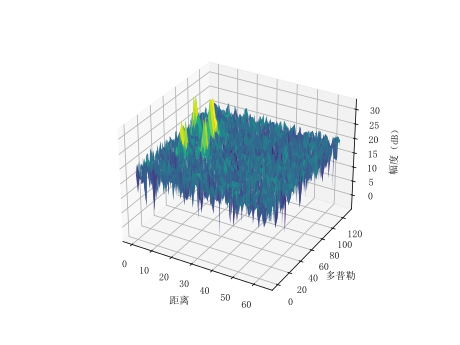
\includegraphics[width = 0.45\linewidth]{figures/4目标/距离多普勒3d.pdf}}
	\subcaptionbox{距离多普勒图\label{距离多普勒图}}{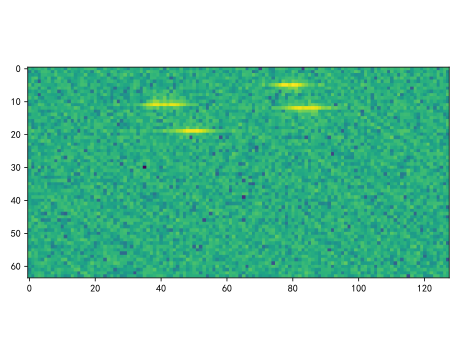
\includegraphics[width = 0.45\linewidth]{figures/4目标/距离多普勒2d.pdf}}
	\caption{四目标距离多普勒图}
	\label{fig:四目标距离多普勒图}
\end{figure}

(4)为验证模型的泛化性,使用在训练集没有出现过的4目标场景进行测试。距离多普勒图如图\ref{fig:四目标距离多普勒图},RA-CFAR检测结果如图\ref{RA-CFAR三维视图}所示,目标点实际分布如图\ref{目标点三维视图}所示。由图可知RA-CFAR在4目标检测场景下仍然保持了较好的检测效果,能够有效地检测出目标点。

\begin{figure}[htbp]
	\centering
	\subcaptionbox{RA-CFAR三维视图\label{RA-CFAR三维视图}}{\includegraphics[width = 0.45\linewidth]{figures/4目标/RA-CFAR3d.pdf}}
	\subcaptionbox{RA-CFAR\label{RA-CFAR}}{\includegraphics[width = 0.45\linewidth]{figures/4目标/RA-CFAR2d.pdf}}
	\subcaptionbox{目标点三维视图\label{目标点三维视图}}{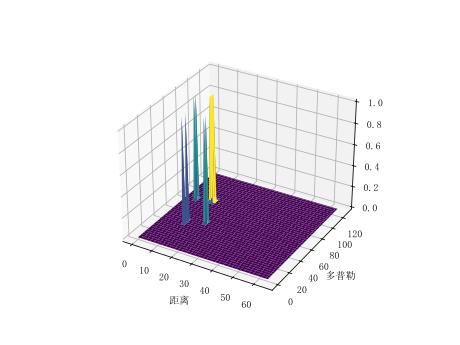
\includegraphics[width = 0.45\linewidth]{figures/4目标/gt3d.pdf}}
	\subcaptionbox{目标点\label{目标点}}{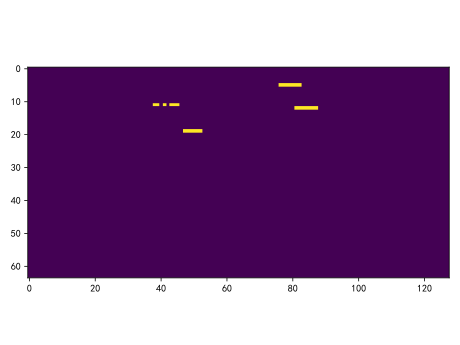
\includegraphics[width = 0.45\linewidth]{figures/4目标/gt2d.pdf}}
	\caption{四目标检测结果}
	\label{fig:四目标检测结果}
\end{figure}

\section{本章小结}
本章分析了当前CFAR算法的问题,发现在大多数情况下CA-CAFR等经典算法,可以有效的检测出目标点。但是面对多目标和较低信噪比情景下存在性能下降以及难以设置参数的问题。而残差神经网络和注意力机制,能够有效地提取和学习不同位置的距离多普勒图的空间特征关联信息,可以准确排除噪声干扰检测出目标点。因此,本章基于此方案设计了基于残差神经网络和十字交叉注意力模块的RA-CFAR方案,与CA-FAR、GOCA-CFAR、SOCA-CFAR、OS-CFAR在多个数据集上进行了对比实验,验证了RA-CFAR方案的有效性。



\chapter{基于多尺度邻域的毫米波点云配准方案}
本章的主要工作内容是优化毫米波雷达点云的迭代配准,通过分析现有配准算法在毫米波雷达点云配准上表示的不足,结合毫米波雷达点云特征,展开相应研究。本章提出了一个结合毫米波雷达多普勒特征以及点云中多尺度邻域特征的特征提取方案以及基于全局特征的配准方案。首先,结合点的多普勒特征以及点的法向量估计提升点云局部特征丰富度;其次,提出了根据多个邻域半径提取多尺度邻域特征的毫米波雷达点云特征提取网络,使用多尺度邻域的融合的方式对抗稀疏性;然后,结合源点云和参考点云特征提出了全局配准参数预测网络,使用提取的全局特征预测一次迭代中的配准参数,加快点云配准的收敛速度;最后,使用提取出的点云特征结合空间坐标进行迭代配准优化。

\section{毫米波雷达点云配准概述}
\subsection{毫米波雷达点云配准问题分析}
随着毫米波雷达点云成像技术在自动驾驶等行业中的广泛运用,毫米波雷达点云配准的准确性与鲁棒性成为研究热点。然而,由于毫米波雷达点云的分辨率低、点云稀疏、以及点云密度不均匀等特点,使得在点云稀疏区域难以有效提取特征,且在密集区域提取的特征不适用于稀疏区,传统的点云刚性配准方法难以有效配准。因此,迫切需要一种能够有效提取毫米波雷达点云特征且适应其分布特征的配准方案。
\subsection{毫米波雷达点云配准方案设计}
基于上述问题分析,本章设计了基于多尺度邻域的毫米波雷达点云配准方案。该方案主要由点级别的领域特征提取网络和全局配置参数预测网络两个部分组成。本章特别关注特征提取的优化,在点级别特征提取中,通过挖掘毫米波雷达点云的多普勒等特征,结合计算点拟合平面估计法向量,引入深度学习网络以提升点云的特征表示能力,克服了无法刚性旋转无法直接用于毫米波雷达点云的缺点,使用点于点的特征关系预测点云配准后位置,从而增强配准效果。在全局特征提取方面,通过拼接两个点云的信息,采用端到端的网络优化配置参数,以加速配准的收敛速度。相对于传统的特征提取方法,深度学习网络的引入有望在全局特征捕捉方面取得更显著的进展,从而使得配准过程更加迅速高效。基于多尺度邻域的毫米波雷达点云配准从毫米波雷达点云数据处理与增强、多尺度邻域特征提取、全局特征提取配准参数预测三个方面完成了配准。主要流程如图\ref{fig:配准流程}所示。


\begin{figure}[htbp]
	\centering
	\includegraphics[width=0.9\linewidth]{figures/配准流程.pdf}
	\caption{配准流程}
	\label{fig:配准流程}
\end{figure}


\section{多毫米波雷达点云配准方案} \label{sec:配准方案整体设计}

% 在点云数据预处理阶段,使用拟合平面法向量的方式丰富点云的局部特征,在点级别特征提取中,结合多普勒特征以及法向量特征使用多尺度邻域的融合的方式对抗稀疏性,提高特征的密度。在全局特征提取阶段以及配准阶段,使用源点云与参考点云的特征拼接,使用配准参数预测网络预测一次迭代中的配准参数,计算点云亲和度,使用预测参数对源点云进行变换加快点云配准的收敛速度,得到变换后的点云,再次提取特征,直到满足迭代次数或者收敛条件。

\subsection{毫米波雷达点云数据处理与增强}
为获取有效标注的点云数据,需要对已知点云数据进行预处理。本方案使用了自采集数据集和Coloradar数据集\cite{ColoRadar}。为了使模型对不同角度、位置和噪声具有鲁棒性,需要对原始点云进行采样和变换,并且从原始点云中分离出源点云和参考点云对源点云进行旋转和平移操作,记录变换矩阵的逆矩阵用于损失的计算。
\par
(1)数据采样。为了增强模型的鲁棒性,采用多种不同的数据增强策略。第一种方式是进行均匀重采样,并打乱点云的顺序;第二种方式是引入高斯噪声,并打乱点云的顺序;第三种方式是进行随机裁剪、均匀重采样、引入高斯噪声,并打乱点云的顺序。这些采样方式的使用旨在模拟不同姿态和位置下的点云变化,提高模型的鲁棒性。
\par
(2)点云分割和随机刚体变换。点将已知点云分割为源点云和目的点云,对源点云加入包括旋转和平移的刚体变换,记录下变换矩阵用于损失的计算。首先,根据一个随机因子,确定旋转和平移的最大幅度。其次,通过生成一个随机的特殊正交群上的旋转矩阵\cite{cuisenaire1999fast},将旋转限制在三维空间内。然后,生成一个在指定范围内均匀分布的随机平移向量。生成的变换参数被组合成一个随机刚性变换矩阵,这个变换矩阵被应用到源点云上,同时确保法向量也受到旋转影响,得到一个变换后的点云。最后,计算这个变换矩阵的逆矩阵和估计矩阵,用于后续的处理,处理过程如图\ref{点云变换}所示。


将点云分割,假设原始点云为 $X$,分割后得到两个点云$P$和$Q$。对点云$P$加入包括旋转和平移的刚体变换,得到旋转矩阵 $R$ 和平移向量$T$。为了叙述简单,接下来的步骤中先忽略平移向量$T$。这一过程可以表示为:

\begin{equation}
P' = PR
\end{equation}

其中,\(P'\) 是经过刚性变换后的点云 \(P\)。
\begin{figure}[htbp]
	\centering
	% Requires \usepackage{graphicx}
	\includegraphics[width=0.96\linewidth]{figures/点云变换.pdf}\\
	\caption{点云刚体变换}
	\label{点云变换}
\end{figure}

为了得到从$P'$到$P$的变换,由公式\eqref{eq:inverse}可知,需要计算旋转矩阵 \(R\) 的逆矩阵 \(R^{-1}\),并记录。
\begin{equation}
	\label{eq:inverse}
P'R^{-1} = PRR^{-1} = P
\end{equation}

逆矩阵的计算公式如\eqref{eq:inverseMatrix}所示,其中,\(R^T\) 表示矩阵 \(R\) 的转置。最终,得到的旋转矩阵的逆矩阵 \(R^{-1}\) 可用于将经过刚性变换后的点云 \(P'\) 还原回原始位置。
\begin{equation}
	\label{eq:inverseMatrix}
R^{-1} = \frac{A^*}{\|R\|}
\end{equation}

数据集处理过程的算法描述如\ref{alg:pointcloudtransform}所示,最终得到的$R^{-1}$就是$P'$与$Q$配准的真实变换,记为$R_{gt}$。
 
\begin{algorithm}[htbp]
	\caption{点云的旋转矩阵计算}
	\label{alg:pointcloudtransform}
	\begin{algorithmic}[1]
		\Require 原始点云 $X$,
		\Ensure 旋转后点云 $P'$, 旋转矩阵的逆矩阵$R^{-1}$
		\State 在$X$中加随机的噪声
		\State 将$X$ 分割为 $P$和$Q$
		\State 在$P$应用旋转和平移矩阵: $P' = RP + T$
		\State 计算旋转矩阵的逆矩阵$R^{-1} = R^T$
		\State \textbf{return} 旋转后的点云 $P'$, 旋转矩阵的逆矩阵 $R^{-1}$
	\end{algorithmic}
\end{algorithm}

(3)法向量估计与PPF计算。点对特征(Points Pairs Features,PPF)\cite{hinterstoisser2016going}是描述两个点之间几何关系的一种表示方法。PPF的结果具有旋转不变形,因为点云配准中的源点云与目的点云之间具有旋转平移的强相关性\cite{5540108},所以PPF结果作为特征能够极大的提升配准效果。PPF的计算基于点的本地几何特性,包括它们的位置和法向量。为了提取点云所在位置的法向量,常见的方案有最小二乘拟合平面求法向量和使用深度图的法向量估计。为了计算速度以及效率的平衡,本方案使用的方法是获取领域内与目标点最近2个点,使用三个点所确定如图\ref{三点平面法向量}所示平面,用此平面法向量代替目标点的法向量。使用KD树如算法\ref{alg:kdtree}所示获取邻域内$k$个点中最近的2个点并且确保这2个点不共线。假点$p_c$设领域内最临近2个点的分别为$p_1,p_2$,从点$p_c$到这两个点的向量为:
\begin{equation}
	\begin{split}
		p_1 - p_c = (x_1 - x_c, y_1 - y_c,z_1 - z_c)\\
		p_2 - p_c = (x_2 - x_c, y_2 - y_c,z_2 - z_c)
	\end{split}
\end{equation}

\begin{figure}[htbp]
	\centering
	% Requires \usepackage{graphicx}
	\includegraphics[width=0.7\textwidth]{figures/三点法向量.pdf}\\
	\caption{点所在平面法向量}
	\label{三点平面法向量}
\end{figure}

因为平面的法向量可以通过平面上的两个非共线向量进行叉乘(向量积)得到,拟合平面的法向量计算公式如\eqref{norm}所示,得到的向量$n$用来代替$p_c$的法向量。
\begin{equation}
	\label{norm}
	n = (p_1 - p_c) \times(p_2 - p_c) 
\end{equation}

假设$p_c,p_1$的法向量分别为$n_c,n_1$,$d = p_1-p_c$,$PPF$运算的公式如\eqref{ppf公式}所示,其中$\|d\|$是向量$d$的模长,$\angle(x, y)$是两个矢量的夹角,且$\angle(x, y) \in [0, \pi]$。

\begin{equation}
	\label{ppf公式}
		PPF(p_c,p_1) = \big(\|d\|^2,\angle(n_c, d),\angle(n_1, d),\angle(n_c, n_1) \big)
\end{equation}



\subsection{基于多尺度邻域的点特征提取}
相比于激光雷达点云,毫米波雷达的点云在精度上往往只能达到厘米级,这导致毫米波雷达的点云稀疏且不均匀,为了挖掘出毫米波雷达点云中点级别更多有意义的特征,本节受到PointNet++的启发,使用多尺度邻域特征融合的方式\cite{qi2017pointnet++},将多个邻域半径邻域的特征融合后作为点的特征表示。

多尺度邻域融合允许网络在不同尺度上获取信息,使其能够更全面、准确地理解点云的结构。采用多尺度邻域融合能够在多个尺度上对点云密度稀疏的局部区域进行特征提取\cite{RJXB202304025},提高特征密度提供更精细的匹配信息,改善点云配准的准确性。在单个邻域半径上,点邻域特征提取网络如图\ref{点特征提取网络}所示,$p_c$为待提取特征的点,假设点$x_c$周围距离不超过阈值$\tau$的邻域内有$k$个点,$p_1,p_2,\cdots,p_k$为邻域点,$\tau$由点云的密度确定。点特征提取网络的输入特征包括每个点的笛卡尔坐标$(x,y,z)$,邻域内每个点$p_i$与$p_c$的坐标差值$\Delta p_{c,i}$,点的极坐标$(\rho,\theta,\sigma)$,以及当前点的多普勒值$d$。$\Delta p_{c,i}$计算公式如\eqref{delta}所示。
\begin{equation}
	\label{delta}
	\Delta p_{c,i} = p_c - p_i
\end{equation}

除以上信息外,使用拟合平面的方式为点$x_c$估计法向量并在提取的特征信息中加入了点$x_c$与领域中每一个点的点对特征计算结果,用于表示点与局部邻域的相关性。


\begin{figure}[htbp]
	\centering
	% Requires \usepackage{graphicx}
	\includegraphics[width=\linewidth]{figures/点特征提取网络.pdf}\\
	\caption{点邻域特征提取网络}
	\label{点特征提取网络}
\end{figure}



假设三个邻域半径的取值为$\tau_1, \tau_2, \tau_3$,多尺度特征提取网络如图\ref{多尺度特征提取网络}所示,图\ref{多尺度特征提取网络}为图\ref{点特征提取网络}分别在三个邻域尺度之上进行迭代特征提取,对提取后的特征进行融合得到点最终的邻域特征。提取点$\tau$邻域特征的步骤如下:
\par 

(1)选取中心点$p_c$以及邻域点$p_1, p_2, \cdots, p_{k-1}$共$K$个点,输入特征为中心点坐标$(x,y,z)$,中心点多普勒$d$,中心点极坐标$(\rho, \theta, \varphi)$,以及通过公式\eqref{norm}选取领域半径。记此时特征向量的维度为$(B,N,C)$,$B$为Batch,$N$为点云中点的数量,$C$为特征通道数,此时$C$如公式\eqref{C1}所示。

\begin{equation}
	\label{C1}
	C_1 = (x,y,z,\rho,\theta,\varphi,d)
\end{equation}
\begin{figure}[htbp]
	\centering
	% Requires \usepackage{graphicx}
	\includegraphics{figures/多尺度特征提取.pdf}\\
	\caption{多尺度特征提取网络}
	\label{多尺度特征提取网络}
\end{figure}

(2)根据邻域半径$\tau$,获取球形邻域内的点计算得到的$\Delta x$,$\Delta y$,$\Delta z$,$PPF(p_1, p_i)$,假设邻域内有$n\_samples$个点,此时得到$n\_samples\times C_2$的特征向量如\eqref{nc2}所示。
\begin{equation}
	\label{nc2}
	\begin{aligned}
		\Delta x_1, \Delta y_1, \Delta &z_1, PPF(p_c, p_1)\\
		\Delta x_2, \Delta y_2, \Delta &z_2, PPF(p_c, p_2)\\
		&\vdots \\
		\Delta x_k, \Delta y_k, \Delta &z_2, PPF(p_c, p_k)
	\end{aligned}
\end{equation}

(3)拼接特征,由于点$p_c$的特征为$1\times7$,为了保证维度的一致性,先把特征向量扩展$(B,N,1,C)$,为了与每个邻域点的特征进行拼接,在新增的第三个维度上复制$n\_samples$次,将$p_c$特征变量扩展为$(B,N,n\_samples,C_1)$,接下来在最后一个维度上拼接邻域特征,得到最终的特征向量为$(B, N, n\_samples, C_1+C_2)$,此时特征通道数为$C=C_1+C_2=14$,特征向量如\eqref{nc12}所示。
\begin{equation}
	\label{nc12}
	\begin{aligned}
	x,y,z,\rho,\theta,\varphi,d,\Delta x_1, &\Delta y_1, \Delta z_1, PPF(p_c, p_1)\\
	x,y,z,\rho,\theta,\varphi,d,\Delta x_2, &\Delta y_2, \Delta z_2, PPF(p_c, p_2)\\
	&\vdots \\
	x,y,z,\rho,\theta,\varphi,d,\Delta x_k, &\Delta y_k, \Delta z_2, PPF(p_c, p_k)
\end{aligned}
\end{equation}

(4)对输入的特征进行二维卷积和池化操作,在图像领域进行二维卷积的时候采用的常见数据格式为$(N,C,H,W)$,N为Batch大小,C为特征通道数,H表示图片的高度,W表示图片的宽度。毫米波雷达点邻域特征提取网络的输入特征为$(B,N,K,C)$,B为Batch大小,N为点云点的数量,K为邻域中点的数量,C为特征通道。在对领域点进行卷积时需要把特征通道放到第二维后进行卷积操作,维度变换后为$(B,C,K,N)$,卷积操作后在第三个维度即邻域点维度做$Max Pooling$。


(5)对多个尺度邻域提取特征进行融合,如图\ref{多尺度特征提取网络}所示。首先选取邻域半径$\tau$的取值,根据经验取邻域半径的列表为$[0.2, 0.4, 0.8]$。依次获取邻域内特征,将所有的特征在最后一个维度进行融合,得到融合后的特征。

\subsection{基于全局特征的配准参数预测}
毫米波雷达点云通常包含复杂的场景和目标,全局特征提取有助于捕捉整个点云的全局结构和一致性信息。同时由于毫米波雷达数据可能受到多路径效应、噪声等因素的影响,通过提取全局特征,可以减小噪声和局部变化等因素对配准结果的干扰提高配准结果的鲁棒性。全局特征提取可以为配准算法提供更好的初始估计。在毫米波雷达点云中,初始估计对于收敛到准确的配准结果非常重要。全局特征可以提供一个更准确的起点,有助于加速配准过程并提高最终配准的精度。全局特征的提取步骤如下:
\par
(1)数据预处理。假设输入的原始点云数据为源点云$P$,参考点云$Q$,每个点云的形状为$(B,J,4)$。B为Batch大小,J为点云大小,4为点云的笛卡尔系坐标加上每个点的多普勒速度值。
由于毫米波雷达原始数据为极坐标系,因此需要用公式\eqref{tocart}把极坐标系转为笛卡尔坐标系。
\begin{equation}
	\label{tocart}
	\begin{aligned}
		x &= \rho \cdot \sin(\theta) \cdot \cos(\varphi) \\
		y &= \rho \cdot \sin(\theta) \cdot \sin(\varphi) \\
		z &= \rho \cdot \cos(\theta)
	\end{aligned}
\end{equation}
为了区分源点云和参考点云,在源点云右侧填充全为0的列,在参考点云在右侧填充全为1的列。


(2)特征提取。全局特征提取网络如图 \ref{全局特征提取网络}所示。特征提取网络采用编码器-池化-解码器的方案。编码器通过五层卷积核为1的卷积层堆叠,将输入数据的特征通道从5维升维到1024维。接下来,使用自适应最大池化,将高维特征映射到固定的维度将最后一维变成1维,保留了最显著的特征。在解码器部分,使用多个全连接层叠加,最后的输出层为$(B,2)$,B为Batch大小,2为输出的$\alpha,\beta$值,用于全局配置参数的设置。
\begin{figure}[htbp]
	\centering
	% Requires \usepackage{graphicx}
	\includegraphics{figures/全局特征提取网络.pdf}\\
	\caption{全局特征提取网络}
	\label{全局特征提取网络}
\end{figure}


\subsection{训练流程}
通过上述数据预处理以及点云特征提取可以得到源点云和参考点云的特征、全局特征、源点云到参考点云的变换$R_{gt},t_{gt}$,训练流程如下:
\par
(1)计算源点云与参考点云的特征距离。使用源点云和参考点云,计算两个点云特征的欧氏距离。在经过特征提取后,源点云和参考点云的特征矩阵分别为$F_{src}$和$F_{ref}$。在三维空间两点$X,Y$之间欧氏距离的计算公式如\eqref{dist}所示。
\begin{equation}
	\label{dist}
	\begin{aligned}
		d &= (x_1-x_2)^2 +  (y_1-y_2)^2 +  (z_1-z_2)^2\\
		&= x_1^2+x_2^2 +  y_1^2+y_2^2  +  z_1^2+z_2^2 - 2x_1x_2 - 2y_1y_2 - 2z_1z_2\\
		&=x_1^2+x_2^2 +  y_1^2+y_2^2  +  z_1^2+z_2^2 - 2(x_1x_2+y_1y_2+z_1z_2)
	\end{aligned}
\end{equation}

把坐标写成向量形式分别为$X=[x_1, y_1, z_1],Y=[x_2,y_2,z_2]$,定义$sum$函数为在最后一个维度上求和,此时距离可以表示为公式\eqref{dist2}。

\begin{equation}
	\label{dist2}
	d = sum(X^2) + sum(Y^2) - 2XY^T
\end{equation}
因此,源点云和参考点云在的特征距离可以表示为公式\eqref{dist3}。

\begin{equation}
	\label{dist3}
	D_{feat} = sum(F_{src}^2) +sum( F_{ref}^2) - 2 F_{src}F_{ref}^T
\end{equation}
\par
(2)计算混合亲和度矩阵。如公式\eqref{affinity}所示,其中$ j $表示源点云中的点的索引,$k $表示参考点云中的点的索引。这个公式反映了特征之间的距离对于初始匹配矩阵值的影响。 $\beta$ 和 $\alpha$ 是预测的参数,它们用于调整特征距离对亲和力的影响。如果 $\alpha$ 是一个浮点数,那么在计算时,所有的距离都会减去相同的 $\alpha$ 值。如果$\alpha$ 是一个向量,那么每个特征点对应的距离都会减去不同的 $\alpha$ 值。$A$是一个形状与特征都和距离矩阵相同的矩阵,但其值已经根据全局参数的预测值预测的参数进行了调整。

\begin{equation}
	\label{affinity}
	A_{jk} = -\beta \cdot (D_{feat}[j,k] - \alpha)
\end{equation}
\par
(3)点匹配概率计算。为了提高数值稳定性以及加快收敛速度,对亲和度矩阵进行Sinkhorn计算\cite{cuturi2013sinkhorn}如算法\ref{alg:sinkhorn}所示,得到归一化的对数概率矩阵。当概率值趋近0或1时,使用对数运算避免了数值下溢或溢出的问题并且在数值优化中往往更容易收敛。然后将对数概率矩阵转换成概率矩阵,该矩阵表示源点与目标点之间的匹配程度。由于概率矩阵表示了每个源点与每个目标点的匹配概率,因此可以使用这些概率来计算加权目标点的坐标。每个源点的加权坐标是目标点的加权平均值,其中权重是与每个目标点相关的匹配概率。概率矩阵中的每一行和每一列都是归一化的,这意味着它们的总和都是1。这使得每个源点都有一个与之相关的匹配概率分布,其中所有概率之和为1,计算过程如算法\ref{alg:sinkhorn}所示。
\begin{algorithm}[htbp]
	\caption{Sinkhorn算法}\label{alg:sinkhorn}
	\begin{algorithmic}[1]
	\Require 对数形式的正矩阵 $log\_alpha$,迭代次数 $n\_iters$,提前终止阈值 $eps$
	\Ensure 双随机矩阵的对数 $log(perm\_matrix)$
	\State 初始化:前一迭代矩阵 $prev\_alpha \leftarrow None$
	\For{$i = 1$ to $n\_iters$}
		\State 行归一化:对每一行的 $log\_alpha$ 进行归一化,使每行元素的指数和为1
		\State 列归一化:对每一列的 $log\_alpha$ 进行归一化,使每列元素的指数和为1
		\If{$eps > 0$ \textbf{and} $prev\_alpha \neq None$}
			\State 计算当前矩阵与前一矩阵的最大绝对差值
			\If{最大差值小于 $eps$}
				\State \textbf{break}
			\EndIf
		\EndIf
		\State 更新 $prev\_alpha$ 为当前的 $log\_alpha$
	\EndFor
	\State \Return $log\_alpha$
	\end{algorithmic}
\end{algorithm}
\par
(4)计算变换。概率矩阵中的每一行和每一列都是归一化的,这意味着它们的总和都是1。这使得每个源点都有一个与之相关的匹配概率分布,其中所有概率之和为1。概率矩阵的每一行都对应于源点云中的一个点,每一列都对应于参考点云中的一个点。虽然最终目标是找出源点云的刚性变换,但是源点云与参考点云可能存在轻微的非刚性形变,通过求加权平均的方式能够缓解非刚性形变,提高配置过程的鲁棒性。将概率矩阵中的每一行与参考点云中的点进行加权求和,从而得到加权的参考点云。
使用源点云和加权参考点云计算两个点云之间的刚性变换。将两个点集分别减去对应的质心,得到质心对齐后的点集,计算质心对齐后的点集之间的协方差矩阵,对协方差矩阵进行SVD分解\cite{kalman1996singularly},得到旋转矩阵如\eqref{旋转公式}所示。根据SVD分解得到的旋转矩阵和质心,计算平移矩阵如\eqref{平移公式}所示。平移矩阵将源点云的质心转移到参考点云的质心位置。

\begin{algorithm}[htbp]
	\caption{计算刚性变换}
	\label{alg:compute_rigid_transform}
	\begin{algorithmic}[1]
		\Require 源点云 $P1$,参考点云 $P2$
		\Ensure 从 $P1$ 到 $P2$ 的旋转矩阵 $R$,平移矩阵 $t$
		\State 计算源点云的质心 $P1_c$ 和参考点云的质心 $P2_c$
		\State  $P1\_centered$ $\gets$  $P1$ -  $P1_c$, $P2\_centered$ $\gets$  $P2$ -  $P2_c$ \Comment{ 将源点云和参考点云中心化}
		\State 计算协方差矩阵 $cov = P1\_centered^\top \cdot P2\_centered $
		\State 计算两个旋转矩阵 $R_{\text{pos}}$ 和 $R_{\text{neg}}$,并选择行列式为正的矩阵
	 \State 计算平移矩阵 $translation = -R \cdot P1_c + P2_c$
		\State 将旋转矩阵和平移矩阵连接起来,得到变换矩阵 $T$
	\end{algorithmic}
\end{algorithm}
(5)设计损失函数。每个迭代步骤,将预测的变换应用到源点云上,并计算与真实变换后的源点云之间的损失。损失函数可以选择为均方误差MSE。
\begin{equation}
	loss = \frac{1}{N}\sum_{j=1}^{N}\| (RP_j+t) - (R_{pred}P_j+t_{pred}) \|^2
\end{equation}
\par
(6)迭代过程。迭代过程中,使用上述损失函数,使用Adam优化器优化学习率设置,学习率为0.0001,批大小为8,训练的epoch数量为1000,使用Early Stopping策略在模型的性能没有提升时提前结束训练。训练过程中使用学习率衰减策略,当模型的性能没有提升时减小学习率。本章模型在训练过程在验证集上各个评估指标的变化曲线如图\ref{fig:验证集评估指标变化曲线}。分析曲线可知,在前50个Epoch各个实验评估指标下降剧烈。在200到300Epoch曲线出现抖动,500Epoch后曲线的趋势开始平稳,模型逐渐收敛。
\begin{figure}[htbp]
	\centering
	\subcaptionbox{MAE(R)}{\includegraphics[width = 0.45\textwidth]{figures/rot_mae_err.pdf}}
	\subcaptionbox{RMSE(R)}{\includegraphics[width = 0.45\textwidth]{figures/rot_rmse_err.pdf}}
	\subcaptionbox{MAE(T)}{\includegraphics[width = 0.45\textwidth]{figures/trans_mae_err.pdf}}
	\subcaptionbox{RMSE(T)}{\includegraphics[width = 0.45\textwidth]{figures/trans_rmse_err.pdf}}
	% \subcaptionbox{Chamfer-Dis}{\includegraphics[width = 0.45\textwidth]{figures/cd.pdf}}
	\caption{验证集评估指标变化曲线}
	\label{fig:验证集评估指标变化曲线}
\end{figure}

\section{实验设计与结果分析}

\subsection{数据采集}
本节使用的数据集为ColoRadar数据集\cite{ColoRadar}和自采集数据集。ColoRadar数据集包含了来自街道,城市,矿山等52个序列超过145分钟的数据。ColoRadar所用毫米波雷达为AWR1843,参数设置如表\ref{第四章雷达参数表}。自采集数据集使用IWR6843采集了包含室内1到3人,室外1到3人的场景,各收集的1000组数据共计6000组数据。
两个数据集所用到的毫米波雷达参数信息如表\ref{第四章雷达参数表}所示。

\begin{table}[htbp]
	\centering
	\tabcolsep=3mm
	\caption{第四章雷达参数表}
	\begin{tabular}{ccc}
		\toprule
		参数 & IWR6843 &AWR1843 \\
		\midrule
		发射天线 & 4 &4 \\
		接收天线 &3 &3  \\
		ADC采样点数 & 128 & 96  \\
		每帧Chrip数 & 128 & 288 \\
		开始频率 &  60.6GHz &  76.9GHz   \\
		带宽 & 2.249GHz &  4GHz  \\
		空闲时间 & 10ns  & 10ns\\
		调频斜率 & 54.725MHz/us& 100MHz/us \\
		\bottomrule
	\end{tabular}
	\label{第四章雷达参数表}
\end{table}

\subsection{实验评估指标}
在刚性变换的评估指标中,平均绝对误差(MAE)、均方误差(MSE)和均方根误差(RMSE)是最常用的评价指标。本节在旋转和平移两个方面使用公式\eqref{MAE}计算平均绝对误差(MAE)使用公式\eqref{RMSE}计算均方根误差(RMSE),得到旋转均方根误差RMSE(R)、旋转平均绝对误差MAE(R)、平移均方根误差RMSE(T)和平移平均绝对误差MAE(T)作为评估指标。除此之外,使用倒角距离(Chamfer-Distance)作为评估指标。倒角距离是一种用于评估两个点云之间的距离的指标,它是两个点云之间的最小距离的平均值。两个点云$X$和$Y$之间的
倒角距离的公式表示为公式\eqref{Chamfer-Distance}所示。倒角距离越小,说明两个点云之间的距离越小,配准效果越好。
\begin{equation}
	\label{Chamfer-Distance}
	\text{Chamfer-Dis}(X,Y) = \frac{1}{|X|} \sum_{x \in X} \min_{y \in Y} \|x - y \|^2 + \frac{1}{|Y|} \sum_{y \in Y} \min_{x \in X} \|x - y \|^2 
\end{equation}
\subsection{消融实验}
为了验证本章加入多普勒特征,拟合法向量,以及多邻域特征提取的有效性,本节设置了对于特征提取部分和多尺度邻域特征提取部分进行了消融实验,通过不同的特征提取方式的组合,对比最终配准效果的各项评估指标,验证本配准方案的有效性。消融实验包含的组合方案有:
\par
(1)网络结构保持不变,在提取特征中去掉法向量。
\par
(2)在提取点邻域特征提取时,只提取固定$\tau$邻域的特征。
\par
(3)网络结构保持不变,在提取特征中去掉多普勒。
\par
(4)本方案,保留了所有的模块。
\par
各模块的组合方式和最终配准结果如表\ref{消融实验}所示。
\
\begin{table}[htbp]
	\centering
	\caption{消融实验}
	\scalebox{0.92}{
		\begin{tabular}{cccccccc}
			\toprule
			多普勒 & 法向量评估 & 多尺度邻域特征&MAE(R) & RMSE(R)& MAE(T) & RMSE(T)& Chamfer-Dis \\
			\midrule
			\Checkmark &  &  \Checkmark& 7.502 & 8.288 & 0.342 & 0.360 & 0.251 \\
			\Checkmark & \Checkmark & & 19.086 & 27.047 & 0.168 & 0.252 &  1.151 \\
			 & \Checkmark & \Checkmark& 7.469 & 21.075 & 0.361 & 0.380 & 0.429 \\
			\Checkmark & \Checkmark & \Checkmark&  6.459 & 6.904 & 0.063 & 0.166 & 0.243 \\
			\bottomrule
		\end{tabular}
	}
	\label{消融实验}
\end{table}
\par
从表\ref{消融实验}可知,添加了多普勒,法向量评估和多尺度邻域特征的配准效果最佳,当保留多普勒和法向量估计去掉多尺度邻域特征后配准效果最差,验证了多尺度邻域特征在配准过程中是至关重要的;当模型去掉多普勒或者去掉法向量评估后,配准精度损失都有了一定的上升,证明了多普勒和法向量评估的必要性;去掉多普勒后平移损失有明显的上升,证明了多普勒信息能够在点云配准中平移变量评估中起到重要作用;去掉法向量评估后平移损失和旋转损失都有明显的上升,证明了法向量评估在旋转矩阵和平移向量的评估上都有贡献。

\subsection{对比实验}
为了验证本章方案的有效性和实验评估的准确性,本节进行了三组对比实验,分别为同类型雷达点云配准实验,不同类型雷达点云配准实验,配准效率对比实验。在这三组实验中本章方法将与 ICP、Go-ICP、 RPM、FGR、 DCP、 PointNetLK、 RPMNet 进行对比。

\par
(1)同类型雷达点云配准实验。为了验证在同类型毫米波雷达点云上训练出的模型配准效果,本节在同一雷达的雷达点云数据集上训练PointNetLK模型,RPMNet模型和本章模型。
\begin{table}[htbp]
	\centering
	\tabcolsep=3mm
	\caption{同类型雷达点云配准实验结果}
	\begin{tabular}{cccccc}
		\toprule
		算法 &  RMSE(R)&MAE(R)& RMSE(T)&MAE(T) & Chamfer-Dis \\
		\midrule
		ICP&24.869&10.003&0.344&0.298&1.088\\
		GoICP&15.905&3.753&0.546&0.176&0.353\\
		RPM&6.907&1.591&0.467&0.183&0.255\\
		FGR&6.729&1.152&0.277&0.274&0.319\\
		PointNetLK&19.416&8.825&0.983&0.524&1.040\\
		DCP&7.435&3.553&0.503&0.344&0.696\\
		RPMNet&6.603&1.312&0.318&0.166&0.243\\
		本方案&6.459&1.204&0.263&0.126&0.180\\
		\bottomrule
	\end{tabular}
	\label{同类型雷达点云配准实验结果}
\end{table}

从表\ref{同类型雷达点云配准实验结果}可以看出,本方案明显优于其余7种算法。与表现最好的RPMNet相比 RMSE(R)降低了2.2\%、MAE(R)降低了8.9\%、 RMSE(T)降低了20.9\%、MAE(T)下降了35\%,证明了使用特征距离代替空间距离对于配准具有明显的提升效果。

(2)不同类型雷达点云配准实验。为了验证在不同毫米波雷达点云上训练出的模型泛化效果,本节在将在AWR1843点云数据集上训练PointNetLK模型,RPMNet模型和本章模型,并且将模型在IWR6843上进行配准使用。初始学习率为0.0001,权值衰减为0.01。


从表\ref{不同类型雷达点云配准实验结果}可以看出,传统算法在不同类型的雷达点云上配准误差没有受到太多的影响,而基于深度学习的算法PonitNetLK和DCP误差率有所上升,PonitNetLK的RMSE(R)、MAE(R)、RMSE(T)、MAE(T)、Chamfer-Dis分别上升了11.3\%、30.3\%、13\%、18.7\%、12.3\%,本方案的RMSE(R)、MAE(R)、RMSE(T)、MAE(T)、Chamfer-Dis分别上升了1.4\%、1.9\%、1.5\%、3.6\%、2.1\%,与其他基于神经网络的模型相比表现更加稳定。推测原因为神经网络在学习特征时在不同类型的点云时,由于毫米波雷达精度、采样频率等参数的不同,导致对于相同物体不同毫米波雷达点云特征有所不同。本方案使用的多尺度邻域特征提取方案能用有效克服优于采样精度和点云放缩带来的特征变化,因此能够维持配准误差的稳定性。

\begin{table}[htbp]
	\centering
	\tabcolsep=3mm
	\caption{不同类型雷达点云配准实验结果}
	\begin{tabular}{cccccc}
		\toprule
		算法 &  RMSE(R)&MAE(R)& RMSE(T)&MAE(T) & Chamfer-Dis \\
		\midrule
		ICP&20.370&10.175&0.097&0.051&1.010\\
		GoICP&16.040&4.037&0.052&0.180&0.353\\
		RPM&8.098&2.081&0.064&0.163&0.325\\
		FGR&7.552&1.465&0.044&0.214&0.184\\
		PointNetLK&21.620&11.499&0.108&0.622&0.168\\
		DCP&7.982&5.160&0.072&0.048&0.954\\
		RPMNet&7.371&2.195&0.521&0.728&0.784\\
		本方案&6.588&0.922&0.064&0.169&0.248\\
		\bottomrule
	\end{tabular}
	\label{不同类型雷达点云配准实验结果}
\end{table}

\par
(3)效率对比实验。为了比较不同的方案在同一点云上的配准速度,本节将计算多个方案分别在AWR1843和IWR6843一帧点云上的配准时间做对比,对比结果如表所示:
\begin{table}[htbp]
	\centering
	\tabcolsep=3mm
	\caption{配准效率对比}
	\scalebox{0.98}{
		\begin{tabular}{ccccccccc}
			\toprule
			点云类型 & ICP & Go-ICP& RPM & FGR & PointNetLK & DCP & RPMNet&本方案 \\
			\midrule
			IWR6843 & 0.032 & 1.85 & 0.047 & 0.043 & 0.062 &0.231 & 0.027 & \textbf{0.022} \\
			AWR1843 & 0.039 & 1.98 & 0.037 & 0.061 & 0.076 &0.331 & 0.042 & \textbf{0.029} \\
			\bottomrule
		\end{tabular}
	}
	\label{配准效率对比实验结果}
\end{table}

\section{本章小结}

本章提出了一种结合毫米波雷达多普勒特征以及点云多尺度邻域特征的特征优化毫米波雷达点云配准方案。在点云数据预处理阶段,通过为毫米波雷达点云数据拟合法平面的方式丰富点级别的空间特征信息;在特征提取阶段,为对抗点云的形变带来的特征变化引入了多普勒信息和多尺度邻域特征提取提高了配准模型的泛化能力和稳定性;在迭代阶段,使用全局特征进行参数预测加快配准的收敛。通过实验分析验证了本方案在多个信噪比、不同目标数量、不同雷达类型的点云上具有优秀的配准效果和泛化能力。
\chapter{原型系统设计与实现}
本文的第三章和第四章提出了基于深度学习的毫米波雷达目标点检测方案和毫米波雷达点云配准方案。本章将介绍如何将这两种方案结合起来,构建一个完整的毫米波雷达点云配准原型系统,并将该系统接入到本课题组研发的校园安防系统中,用于多毫米波雷达场景的毫米波雷达点云数据融合,并且用融合后的数据进行目标检测和跟踪。本章将从系统整体设计、系统实现、系统测试三个方面介绍原型系统的设计和实现。
\section{系统设计}
\subsection{系统架构}
基于本文第三章和第四章提出的毫米波雷达目标点检测方案和毫米波雷达点云配准方案,本文将设计一个完整的毫米波雷达点云配准原型系统。系统的整体架构如图\ref{fig:系统架构}所示。
\begin{figure}[htbp]
    \centering
    \includegraphics[width=0.9\linewidth]{figures/系统架构.pdf}
    \caption{系统架构}
    \label{fig:系统架构}
\end{figure}
\par
本系统主要分为雷达层、数据采集层,数据存储层、点云处理层、规则层和应用层。雷达层由多个IWR6843毫米波雷达组成,负责环境检测并将回波信号转换为二进制数据传输给数据采集层。数据采集层主要负责接收雷达层传来的二进制数据,将二进制数据转换为点云数据,然后将点云数据存储到数据存储层。数据存储层主要负责存储数据采集层传来的点云数据和规则层设置的规则参数。点云处理层主要负责接收数据存储层传来的点云数据,然后对点云数据进行处理,包括点云的预处理、待配准点云的选择、点云的配准。规则层主要负责接收点云处理层传来的配准后的点云数据,根据预先设定的规则判断点云数据是否满足规则,如果满足规则将触发的规则传给应用层。应用层主要负责接收规则层传来的触发的规则,根据触发的规则进行相应的处理,包括将点云数据传给目标检测和跟踪模块,将点云数据传给数据融合模块等。
\subsection{系统详细设计}

\par
(1)雷达层
\par
雷达层由多个IWR6843毫米波雷达组成,负责环境检测并将回波信号转换为二进制数据传输给数据采集层。IWR6843毫米波雷达是德州仪器公司推出的一款毫米波雷达,工作频率为60GHz,具有高分辨率、高精度、高灵敏度等特点。IWR6843毫米波雷达可以通过SPI接口将回波信号转换为二进制数据传输给数据采集层。

\par
(2)数据采集层
\par
数据采集层负责接收雷达层传来的二进制数据,由数据采集模块、数据处理模块和目标点检测模块组成。数据采集模块负责接收雷达层传来的实时二进制数据。为了保证目标检测的实时性以及系统的健壮性,在数据采集模块以及数据处理模块之间使用消息队列进行解耦,通过异步处理的方式进行削峰填谷提升歘同的吞吐量,根据雷达设备的ID,作为消息队列的topic,将数据采集模块采集到的数据发送到消息队列中过程如图\ref{fig:数据采集模块}所示。数据处理模块负责接收数据采集模块传来的二进制数据,然后对二进制数据进行处理,将二进制数据转换为点云数据。目标点检测模块负责接收数据处理模块传来的点云数据,然后对点云数据进行目标点检测。数据采集层的处理过程如图\ref{fig:采集模块处理过程}所示。
\begin{figure}[htbp]
    \centering
    \includegraphics[width=0.9\linewidth]{figures/数据采集模块.pdf}
    \caption{数据采集模块}
    \label{fig:数据采集模块}
\end{figure}

\begin{figure}[htbp]
    \centering
    \includegraphics[width=0.9\linewidth]{figures/采集模块处理过程.pdf}
    \caption{采集模块处理过程}
    \label{fig:采集模块处理过程}
\end{figure}

\par
(3)数据存储层
\par
数据存储层主要负责存储数据采集层传来的点云数据,主要由MySQL、MongoDB、Redis、HDFS等数据库组成,负责存储点云数据。MongoDB负责存储点云数据的原始数据;MySQL负责存储经过目标点检测的点云数据和经过点云配准的点云数据;Redis负责储存上层规则的缓存;HDFS负责存储预训练的目标点检测模型和配准模型。

\par
(4)点云处理层
\par
点云处理层主要负责接收数据存储层传来的点云数据,然后对点云数据进行处理,点云处理层主要由点云选择模块、点云配准模块组成。点云选择模块负责选择待配准的点云数据,包括选择待配准的点云数据的时间、选择待配准的点云数据的空间等;点云配准模块负责对待配准的点云数据进行配准,包括点云的特征提取、点云的特征匹配、点云的配准等,如图\ref{fig:点云处理层}所示。

\begin{figure}[htbp]
    \centering
    \includegraphics[width=0.6\linewidth]{figures/点云处理层.pdf}
    \caption{点云处理层}
    \label{fig:点云处理层}
\end{figure}

\par
(5)规则层
\par
规则层主要负责接收点云处理层传来的配准后的点云数据,然后根据预先设定的规则判断点云数据是否满足规则,如果满足规则将触发的规则传给应用层。规则层主要由原子规则模块、组合规则模块、规则引擎模块组成。原子规则模块负责定义原子规则;组合规则模块负责定义组合规则,对规则进行交集或者并集的操作;规则引擎模块负责根据原子规则和组合规则判断点云数据是否满足规则,如图\ref{fig:规则层}所示。

\begin{figure}[htbp]
    \centering
    \includegraphics[width=0.6\linewidth]{figures/规则层.pdf}
    \caption{规则层}
    \label{fig:规则层}
\end{figure}

\par
(6)应用层
\par
应用层主要负责接收规则层传来的触发的规则,然后根据触发的规则进行相应的处理,包括将点云数据传给目标检测和跟踪模块,经检测到的目标轨迹传给可视化挂机模块等。应用层主要由目标检测和跟踪模块、可视化模块、报警模块组成。目标检测和跟踪模块负责接收点云数据,然后对点云数据进行目标检测和跟踪,最后将检测到的目标轨迹传给可视化模块;可视化模块负责接收目标检测和跟踪模块传来的目标轨迹,然后将目标轨迹可视化;报警模块负责接收规则层传来的触发的规则,然后根据触发的规则进行报警。
\section{系统测试}
\subsection{系统测试环境}
本节给出了原型系统部署的硬件环境和软件环境,如表\ref{硬件配置表}和表\ref{软件配置表}所示。
\par
(1)硬件环境
\par
\begin{table}[htbp]
	\centering
	\tabcolsep=3mm
	\caption{硬件配置表}
	\begin{tabular}{cccp{3cm}}
		\toprule
		设备 & 参数 &数量&用途 \\
		\midrule
		联想 ThinkStation P340 & \makecell[l]{内存:32G \\ 硬盘:2T \\ 显卡:GTX 1660 Super \\ CPU: Intel i7-11500} &1 & 部署校园安防系统以及点云检测和配准模块 \\
        IWR6843毫米波雷达 & \makecell[l]{发射天线:4 \\ 接收天线:3 \\ 开始频率:60.6GHz \\ 带宽: 2.249GHz} &3 & 环境感知 \\
        DCA1000 EVM & /  &3 & 采集数据 \\
		\bottomrule
	\end{tabular}
	\label{硬件配置表}
\end{table}

\par
(2)软件环境
使用Torch进行模型部署,MySQL存储包括规则信息、报警信息等业务信息,MongoDB负责存储点云数据的原始数据,JMETER进行大量雷达数据的压测。
\par
\begin{table}[htbp]
	\centering
	\tabcolsep=2cm
	\caption{软件配置表}
	\begin{tabular}{cc}
		\toprule
		软件 & 版本 \\
		\midrule
		Python & 3.10.13 \\
        Torch & 2.2.0  \\
        MySQL & 8.0.28 \\
        MongoDB & 5.0.5 \\
        Apache JMETER & 5.4.1 \\
		\bottomrule
	\end{tabular}
	\label{软件配置表}
\end{table}

\subsection{系统功能测试}
为了确保毫米波雷达点云配准原型系统的功能正常,本节进行了系统功能测试。系统功能测试主要包括点云数据采集功能测试、点云数据存储功能测试、点云数据处理功能测试、规则判断功能测试、目标检测和跟踪功能测试、可视化功能测试、报警功能测试等。本节将对与毫米波雷达点云检测与配准相关的功能,添加毫米波雷设备、点云数据采集、目标检测和跟踪功能的测试过程展开详细描述。完整系统功能测试的测试用例如表\ref{系统功能测试用例}所示。
\begin{table}
    \centering
    \tabcolsep=3mm
    \caption{系统功能测试用例}
    \begin{tabular}{ccp{3cm}c}
        \toprule
        测试用例编号 & 测试用例名称 & 预期结果 & 测试结果 \\
        \midrule
        0 & 添加雷达设备测试 & 雷达层能够在指定位置正确添加雷达设备& 通过 \\
        1 & 点云数据采集功能测试 & 数据采集模块能够正常接收雷达层传来的二进制数据 & 通过 \\
        2 & 点云数据存储功能测试 & 数据存储层能够正常存储数据采集层传来的点云数据 & 通过 \\
        3 & 点云数据处理功能测试 & 点云处理层能够正常接收数据存储层传来的点云数据 & 通过 \\
        4 & 规则判断功能测试 & 规则层能够正常判断点云数据是否满足规则 & 通过 \\
        5 & 目标检测和跟踪功能测试 & 目标检测和跟踪模块能够根据点云数据检测到目标并且跟踪目标轨迹 & 通过 \\
        6 & 可视化功能测试 & 可视化模块能够正常接收目标检测和跟踪模块传来的目标轨迹 & 通过 \\
        7 & 报警功能测试 & 报警模块能够正常接收规则层传来的触发的规则 & 通过 \\

        \bottomrule
    \end{tabular}
    \label{系统功能测试用例}
\end{table}

\par
(1)添加雷达设备测试
\par
添加雷达设备测试主要测试雷达层能否在指定位置正确添加雷达设备,使用指定的雷达SN号和雷达位置添加雷达设备,然后检查雷达设备是否添加成功。
\begin{figure}[htbp]
    \centering
    \subcaptionbox{添加雷达设备}{\includegraphics[width = 0.49\linewidth]{images/添加雷达设备.png}}
    \subcaptionbox{管理雷达设备}{\includegraphics[width = 0.49\linewidth]{images/管理雷达设备.png}}
    \caption{添加雷达设备测试}
    \label{fig:添加雷达设备测试}    
\end{figure}
\par
(2)点云数据采集功能测试
\par
点云数据采集功能测试主要测试数据采集模块是否能够正常接收雷达层传来的二进制数据,数据处理模块是否能够正常接收数据采集模块传来的二进制数据,目标点检测模块是否能够正常接收数据处理模块传来的点云数据,点云数据采集模块过滤后的点云如图\ref{fig:点云数据采集功能测试}所示。
\begin{figure}[htbp]
    \centering
    \includegraphics[width = 0.8\linewidth]{images/点云数据.png}
    \caption{点云数据采集功能测试}
    \label{fig:点云数据采集功能测试}    
\end{figure}

\par
(3)目标检测和跟踪功能测试
\par
收到点云数据后,目标检测模块根据点云数据检测到目标后,跟踪目标移动,使用目标移动的历史轨迹,绘制目标移动轨迹图,并将轨迹图传给可视化模块和存储模块。目标检测和目标轨迹绘制的效果分别如图\ref{目标检测}和\ref{目标历史轨迹}所示。

\begin{figure}[htbp]
    \centering
    \subcaptionbox{目标检测 \label{目标检测} }{\includegraphics[width = 0.45\linewidth]{images/目标检测.png}}
    \subcaptionbox{目标历史轨迹 \label{目标历史轨迹}}{\includegraphics[width = 0.48\linewidth]{images/轨迹回放.png}}
    \caption{目标检测和跟踪功能}
    \label{fig:目标检测和跟踪功能}    
\end{figure}
\par

\subsection{系统性能测试}
\par
(1)点云提取与配准效率测试
\par
毫米波雷达工作时,平均每秒会发送7帧数据,需要对每帧数据提取出点云并根据选的点云进行配准。由于目标追踪的实时性要求,需要及时消费发往消息队列的数据,因此需要对点云提取与配准的效率进行测试。通过脚本向消息队列发送数据,模拟雷达数量增加的负载情况,点云配准模块的配准速率,检测提取与配准的效率。如图\ref{fig:效率测试}所示,随着雷达数量的增加点云提取与配准的响应时间在增加,但是仍在0.01秒以下,效率仍然能够满足实时性的要求。

\begin{figure}[htbp]
    \centering
    \includegraphics[width = 0.6\linewidth]{figures/效率测试.pdf}
    \caption{效率测试}
    \label{fig:效率测试}    
\end{figure}

(2)配准后点云目标识别准确度测试
\par
为了验证配准后点云的目标识别效果,采集了2个雷达运行1小时的数据,共75600条,其中有目标的数据为15138条,对这些配准后的点云数据进行目标识别,目标识别结果分类如图\ref{目标识别结果分类}所示,统计结果如表\ref{目标识别统计}所示。配准后的点云数据的目标检测准确率达到了96.43\%,精确率达到了92.26\%,召回率达到了96.92\%,说明配准后的点云数据的目标识别效果较好。

\begin{table}[htbp]
    \centering
    \tabcolsep=5mm
    \caption{目标识别结果分类}
    \begin{tabular}{ccc}
        \toprule
        \diagbox{真实}{预测} & 有目标 & 无目标 \\
        \midrule
        有目标 & 14673 & 465 \\
        无目标 & 1231 &  58231 \\
        \bottomrule
    \end{tabular}
    \label{目标识别结果分类}
\end{table}

\begin{table}[htbp]
    \centering
    \tabcolsep=1cm
    \caption{目标识别统计}
    \begin{tabular}{cc}
        \toprule
        评估指标 & 评估值 \\
        \midrule
        有目标数量 & 15138 \\
        无目标数量 & 60462 \\
        准确率 & 96.43\% \\
        精确率 & 92.26\% \\
        召回率 & 96.92\% \\
        \bottomrule
    \end{tabular}
    \label{目标识别统计}
\end{table}
\section{本章小结}
本章主要介绍了基于本文第三章和第四章提出的毫米波雷达目标点检测方案和毫米波雷达点云配准方案构建的一个完整的毫米波雷达点云配准原型系统,并将该系统接入到本课题组研发的校园安防系统中,用于多毫米波雷达场景的毫米波雷达点云数据融合,并且用融合后的数据进行目标检测和跟踪。本章从系统整体设计、系统实现、系统测试三个方面介绍原型系统的设计和实现,验证了毫米波雷达点云检测与配准方案的可行性。


\chapter{总结与展望}
\section{本文工作总结}
为了解决毫米波雷达点云在应用过程中的目标点检测与配准问题,本文深入分析了毫米波雷达数据在目标点检测和配准两个阶段的特点和难点,完成了以下工作:
\par
(1) 针对毫米波雷达工作中易受到噪声干扰,而恒虚警率算法在低信噪比、多目标的情况下无法有效检测目标点的问题,提出了一种基于残差神经网络的目标点提取方案。使用多层残差块提取距离多普勒图全局特征,引入十字交叉注意力机制着重关注距离多普勒图中目标点所在位置行和列的特征,帮助模型更有效地提取位置信息捕捉空间位置关联性。与其他常用算法通过实验对比,验证了方案的适用性和有效性。
\par
(2) 针对毫米波雷达点云密度稀疏且不均匀,导致传统配准算法难以工作的问题,提出使用多尺度邻域的特征提距离代替空间距离的方案,并使用拟合法向量、多普勒信息提取等方式进一步丰富了邻域特征。为了避免初始值设置不当导致配准难以收敛的问题,通过全局特征推测配准初始值并且在每次迭代后优化配准参数。实验结果表明,与同类方案相比本方案的 RMSE(R)、MAE(R)、RMSE(T)、MAE(T)分别降低了2.2\%、8.9\%、 20.9\%、35\%。
\par
(3) 为了验证本文提出方案在落地场景中的有效性,搭建了原型系统并且集成进现有的校园安防平台,用于多毫米波雷达场景的毫米波雷达点云数据融合,并且用融合后的数据进行目标检测和跟踪。验证了本方案的有效性和实用性。
\section{未来工作展望}
本文针对毫米波雷达距离多普勒图目标点检测和点云配准问题进行了探索,给出了一些解决方案,但是还有很多工作可以继续深入研究:
\par
(1) 本文采取了分析距离多普勒图的方式进行目标点提取,考虑到多帧距离多普勒图在时间序列上具有连续性,因此未来可以考虑使用时序模型结合当前帧的距离多普勒图进行目标点提取。
\par
(2) 本文提出了基于多尺度邻域的特征提取方案,但是在实际应用中,如果选择的邻域半径过多,会导致特征提取方案的计算量较大,因此未来需要一个邻域半径选择方案,辅助多尺度邻域特征提取。


\iffalse
% xdus 已经实现下面文件的引用
% 为了使语法提示正确工作,在这里引用但是不编译
% 随着毫米波雷达点云成像技术在自动驾驶、医疗成像、地形测绘等领域的大量使用,毫米波雷达点云检测与多点云配准作为重要步骤,其精确度有了更高的要求。然而,在低信噪比、多目标的情况下,使用恒虚警率(CFAR)算法检测毫米波雷达点云时,存在性能退化和无法有效检测出目标点的问题。此外,由于毫米波雷达点云具有低分辨率、稀疏性、密度分布不均匀的特点,存在无法有效提取点特征和点云较稠密处提取的特征在稀疏处不适用的问题,传统的点云配准方法在其应用中面临严峻挑战。因此,本文聚焦毫米波雷达点云检测与配准,具体研究工作如下:

% 毫米波雷达点云成像技术在自动驾驶、医疗成像、地形测绘等领域发挥着重要作用,雷达目标点检测与多点云配准是其重要组成部分。由于毫米波雷达工作频率低、噪声干扰大,其点云具有低分辨率、稀疏性、密度分布不均匀的特点,这些特点导致无法有效检测毫米波雷达目标点且多毫米波雷达点云难以精确配准。本文聚焦毫米波雷达点云检测与配准,基于毫米波雷达距离多普勒图特征和多毫米波雷达点云多尺度邻域特征,研究毫米波雷达目标点检测方案和毫米波雷达点云精确配准方案,有效提升了目标点检测准确度与多毫米波雷达点云配准精度。

毫米波雷达点云成像技术在自动驾驶、医疗成像、地形测绘等领域发挥着重要作用,雷达目标点检测与多点云配准是其重要组成部分。然而,由于毫米波雷达的工作频率较低且易受噪声干扰,其产生的点云分辨率较低、稀疏且密度分布不均,导致难以有效检测目标点和多点云难以精确配准。本文聚焦毫米波雷达点云检测与配准,基于毫米波雷达距离多普勒图特征和多毫米波雷达点云多尺度邻域特征,研究毫米波雷达目标点检测方案和毫米波雷达点云精确配准方案,有效提升了目标点检测准确度与多毫米波雷达点云配准精度。

\par
针对恒虚警率检测算法在低信噪比、多目标的情况下无法有效检测出目标点的问题,提出一种基于残差神经网络的距离多普勒图目标点检测方案RA-CFAR。通过多层残差块提取距离多普勒图全局特征进行全局噪声评估,引入了自注意力模块捕捉距离多普勒图峰值区域的空间位置相关性,克服距离多普勒图中目标点位置的旁瓣效应。在公开数据集以及自建数据集上将本方案与多种常用恒虚警率检测算法进行对比,结果表明,相较于CA-CFAR、SOCA-CFAR、GOCA-CFAR、OS-CFAR,在低信噪比情况下AUC值分别提升了4\%、8\%、11.9\%、29.4\%;在多目标情况下AUC值分别提升了2.29\%、2.71\%、3.36\%、7.19\%。
\par
针对无法有效提取点特征和点云较稠密处提取的特征在稀疏处不适用的问题,提出基于多尺度邻域的特征提取方案。在预处理阶段引入KD树计算邻域内的邻近点辅助拟合点云邻域平面,使用拟合平面法向量作为点云法向量的方式增加邻域信息丰富度。在特征提取阶段为了提升特征在不同稀疏区域的适用性,结合多普勒信息、拟合法向量和空间坐标信息,在多个$\tau$尺寸的邻域上提取特征合并作为点特征对抗点云的稀疏和不均匀性。在配准阶段使用特征距离代替空间距离增强配准算法的鲁棒性,通过全局特征推测配准初始值,并且在每次迭代后优化配准参数,避免初始值设置不当导致配准难以收敛的问题。实验结果表明,与同类方案相比本方案的 RMSE(R)、MAE(R)、RMSE(T)、MAE(T)分别降低了2.2\%、8.9\%、 20.9\%、35\%。

以上研究内容均在毫米波雷达公开数据集以及自建数据集上通过检测率和配准损失率等评估指标进行了实验验证,实验结果表明,本文提出的毫米波雷达点云配准方案在低信噪比、多目标、稀疏性、密度分布不均匀等情况下均表现出优异的性能。
Millimeter-wave radar point cloud imaging technology plays a significant role in fields such as autonomous driving, medical imaging, and terrain mapping. Radar target point detection and multi-point cloud registration are crucial steps in its application. Due to the low working frequency and high noise interference of millimeter-wave radar, its point clouds are characterized by low resolution, sparsity, and uneven density distribution. These characteristics lead to ineffective detection of millimeter-wave radar target points and difficulties in precise registration of multiple millimeter-wave radar point clouds. This thesis focuses on millimeter-wave radar point cloud detection and registration. Based on the features of millimeter-wave radar range-Doppler maps and the multi-scale neighborhood features of multiple millimeter-wave radar point clouds, this study explores millimeter-wave radar target point detection schemes and precise registration schemes for millimeter-wave radar point clouds, effectively improving the accuracy of target point detection and the precision of multi-millimeter-wave radar point cloud registration.

Addressing the issue that the Constant False Alarm Rate (CFAR) algorithm cannot effectively detect target points under low signal-to-noise ratios and multiple target scenarios, this thesis proposes a Distance-Doppler map target point detection scheme based on Residual Neural Networks, named RA-CFAR. Through extracting global features from distance-Doppler maps using multi-layer residual blocks for global noise assessment, this scheme introduces a self-attention module to capture the spatial location relevance of the peak areas in the distance-Doppler maps, overcoming the sidelobe effects of target point locations within the maps. Comparisons with CA-CFAR、SOCA-CFAR、GOCA-CFAR and OS-CFAR on public datasets and proprietary datasets demonstrate that, in low signal-to-noise ratio scenarios, the Area Under the Curve (AUC) values increased by 4\%, 8\%, 11.9\%, and 29.4\% respectively; in multi-target scenarios, the AUC values increased by 2.2\%, 2.71\%, 3.36\%, and 7.19\% respectively.

In response to the problem of ineffective point feature extraction and the inapplicability of features extracted in denser areas of point clouds in sparser areas, this thesis proposes a feature extraction scheme based on multi-scale neighborhoods. In the preprocessing stage, a KD-tree is introduced to calculate nearby points within the neighborhood to assist in fitting the plane of the point cloud neighborhood. The fitted plane's normal vector is used as the point cloud's normal vector to enrich neighborhood information. During the feature extraction stage, to improve the applicability of features in different sparse regions, features are extracted and combined as point characteristics on multiple neighborhoods of different $\tau$ sizes, integrating Doppler information, fitted normal vectors, and spatial coordinates. In the registration phase, feature distance replaces spatial distance to enhance the robustness of the registration algorithm. Global features are used to estimate initial registration values, and registration parameters are optimized after each iteration to avoid issues with registration convergence caused by improper initial value settings. Experimental results demonstrate that, compared to similar schemes, the proposed solution has reduced RMSE(R), MAE(R), RMSE(T), and MAE(T) by 2.2\%, 8.9\%, 20.9\%, and 35\%, respectively.

The research content discussed has been experimentally validated on public millimeter-wave radar datasets and proprietary datasets through evaluation metrics such as detection rate and registration loss rate. The results indicate that the millimeter-wave radar point cloud registration scheme proposed in this thesis exhibits excellent performance in scenarios with low signal-to-noise ratios, multiple targets, sparsity, and uneven density distribution.
\begin{center}
    {
    \zihao{-4}
    \renewcommand{\arraystretch}{1.28}
    \begin{tabular}{p{4cm}l}
        符号 & 符号名称 \\
        $\pi$ & 圆周率 \\
        $\phi$ & 相位 \\
        $S$ & Chrip斜率\\
        $c$ & 光速 \\
        $B$ & Chrip带宽 \\
        $T_c$ & Chrip发送间隔 \\
        $\Delta\Phi$ & Chrip相位差 \\
        $\Delta f$ & Chrip频率差 \\
        $\Delta t$ & Chrip时间差 \\
        $S_r(t)$ & Chrip接收信号 \\
        $S_s(t)$ & Chrip发送信号 \\
        $P_t(t)$ & 发送信号相位 \\
        $P_r(t)$ & 接收信号相位 \\
        $Z_{CZ}$ & 单元平均值 \\
        $\rho$&  极轴长度\\
        $P$ & 源点云 \\
        $Q$&  参考点云\\
    \end{tabular}
    }

\end{center}


\begin{center}
{
\zihao{-4}
\renewcommand{\arraystretch}{1.28}
\begin{tabular}{p{2.5cm}p{6cm}l}
    缩略语 & 英文全称 &  中文对照 \\
    CA-CFAR &  Cell Average CFAR& 单元平均恒虚警率\\
    CFAR &Constant False Alarm Rate &恒虚警率\\
    CNN & Convolutional Neural Network & 卷积神经网络 \\
    CUT & Cell Under Test & 测试单元\\
    FFT & Fast Fourier Transform & 快速傅里叶变换 \\
    FMCW & Frequency Modulated Continuous Wave & 调频连续波 \\
    GO-CFAR &  Greatest of CFAR & 单元平均选大恒虚警率\\
    IF & Intermediate Frequency & 中频 \\
    MAE & Mean Absolute Error & 平均绝对误差\\
    MSE& Mean Square Error& 均方误差\\
    MLP&  Multi-layer Perceptron & 多层感知机\\
    OS-CFAR &  Ordered Statistic CFAR & 有序统计恒虚警率\\
    PPF & Point Pair Feature & 点对特征\\
    RA-CFAR &  Residual Attention CFAR & 残差自注意力恒虚警率\\
    RMSE & Root Mean Square Error & 均方根误差\\
    RX & Receiving Antenna & 接收天线\\
    SO-CFAR &  Smallest of CFAR & 单元平均选小恒虚警率\\
    SNR & Signal to Noise Ratio & 信噪比\\
    SVD & Singular Value Decomposition & 奇异值分解\\
    TX & Transmitting Antenna & 发射天线\\
\end{tabular}
}
\end{center}
\section{基本情况} \anon{赵文超},\anon{男},\anon{河南周口人},\anon[XXX ]{1997年12月出生},\anon[XXX ]{西安电子科技大学}\anon[XXX ]{广州研究院}\anon{计算机技术}专业2021级硕士研究生。 
\section{教育背景}
\begin{edubg}
\anon{2017.09~2021.07} & \anon{河南工业大学},本科,专业:\anon{软件工程}\\
\anon{2021.09~ }& \anon{西安电子科技大学},硕士研究生,专业:\anon{计算机技术}\\
\end{edubg}
\section{攻读硕士学位期间的研究成果}
\subsection{申请(授权)专利}
\begin{resresult}
	\item \anon[(第一学生发明人)]{祝幸辉, \textbf{\anon{赵文超}}, 沈玉龙等}.一种基于深度学习的毫米波雷达点云数据迭代配准方法:中国, CN202410300316.6
\end{resresult}

\subsection{参与科研项目及获奖}
\begin{resresult}
	\item 国家重点研发计划, 智慧城市云计算平台及服务关键技术研究, 2019.12-2022.11, 结题, 参与。
	\item 国家自然科学基金, 多域物联网系统数据安全关键技术研究, 2023.01-2027.12, 在研, 参与。
	\item 企、事业单位委托项目, 校园安防智慧哨兵系统, 2021.06-2024.07, 结题, 研发负责人。

\end{resresult}

时光飞逝,转眼间已到毕业之际。在这三年间遇到了许多良师益友,他们对我的工作和学习提供许多帮助,在此,我要向这些人表达最真挚的感谢和敬意。

首先,我要感谢沈玉龙老师,沈老师严谨的科研态度,塑造了良好的实验室氛围;沈老师为实验室提供了优越的实验条件和充足的实验设备,并经常组织学术讲座,极大的开拓了我的专业视野。感谢祝幸辉老师,研究生三年,祝老师亦师亦友,在工作和学习上为我提供了许多关心和帮助;在学习和科研上,祝老师为我指明了方向让我能够继续探索;在生活上他所传授丰富的阅历让我不断地成长。

感谢实验室的所有老师和同学,感谢他们的帮助为我的研究带来了许多启发与灵感。感谢师兄师姐刘太鹏、匡昶、孙俊飞、邱和龙、王凯、王海洋、张翰霆、王娟、严静、张潇丹,为我了科研和工作提供了许多指导,让我少走了许多弯路。感谢同门毛佳、吕龙龙、曹强、冯林林、张启元、田泽中、窦俊、顾书浩、童伟,有他们陪伴、帮助和支持,让我的研究生生活充满乐趣。感谢师弟师妹罗文勋、杨丽、陈鸿林、文金铭、梁家杰、滕少西,感谢他们在我找工作以及写论文时承担项目,让我没有后顾之忧。感谢我的朋友谢亦高、张智嵩、陈健航,在我读研期间的鼓励以及帮助,让我更有勇气坚持下去。

感谢我的家人,在我多年的求学中生涯中,家人的无条件支持和付出永远是我最坚实的后盾和最温暖的港湾。

感谢所有曾为我提供过帮助与支持的人。感谢以上所有提及的人,还要感谢那些虽然没被提及但是对我有过帮助的人,虽未提及但是我会永远记得你们的帮助,谢谢你们!


\bibliography{chapters/references}
\fi


\end{document}
